\documentclass[11pt]{article}

    \usepackage[breakable]{tcolorbox}
    \usepackage{parskip} % Stop auto-indenting (to mimic markdown behaviour)
    
    \usepackage{iftex}
    \ifPDFTeX
    	\usepackage[T1]{fontenc}
    	\usepackage{mathpazo}
    \else
    	\usepackage{fontspec}
    \fi

    % Basic figure setup, for now with no caption control since it's done
    % automatically by Pandoc (which extracts ![](path) syntax from Markdown).
    \usepackage{graphicx}
    % Maintain compatibility with old templates. Remove in nbconvert 6.0
    \let\Oldincludegraphics\includegraphics
    % Ensure that by default, figures have no caption (until we provide a
    % proper Figure object with a Caption API and a way to capture that
    % in the conversion process - todo).
    \usepackage{caption}
    \DeclareCaptionFormat{nocaption}{}
    \captionsetup{format=nocaption,aboveskip=0pt,belowskip=0pt}

    \usepackage[Export]{adjustbox} % Used to constrain images to a maximum size
    \adjustboxset{max size={0.9\linewidth}{0.9\paperheight}}
    \usepackage{float}
    \floatplacement{figure}{H} % forces figures to be placed at the correct location
    \usepackage{xcolor} % Allow colors to be defined
    \usepackage{enumerate} % Needed for markdown enumerations to work
    \usepackage{geometry} % Used to adjust the document margins
    \usepackage{amsmath} % Equations
    \usepackage{amssymb} % Equations
    \usepackage{textcomp} % defines textquotesingle
    % Hack from http://tex.stackexchange.com/a/47451/13684:
    \AtBeginDocument{%
        \def\PYZsq{\textquotesingle}% Upright quotes in Pygmentized code
    }
    \usepackage{upquote} % Upright quotes for verbatim code
    \usepackage{eurosym} % defines \euro
    \usepackage[mathletters]{ucs} % Extended unicode (utf-8) support
    \usepackage{fancyvrb} % verbatim replacement that allows latex
    \usepackage{grffile} % extends the file name processing of package graphics 
                         % to support a larger range
    \makeatletter % fix for grffile with XeLaTeX
    \def\Gread@@xetex#1{%
      \IfFileExists{"\Gin@base".bb}%
      {\Gread@eps{\Gin@base.bb}}%
      {\Gread@@xetex@aux#1}%
    }
    \makeatother

    % The hyperref package gives us a pdf with properly built
    % internal navigation ('pdf bookmarks' for the table of contents,
    % internal cross-reference links, web links for URLs, etc.)
    \usepackage{hyperref}
    % The default LaTeX title has an obnoxious amount of whitespace. By default,
    % titling removes some of it. It also provides customization options.
    \usepackage{titling}
    \usepackage{longtable} % longtable support required by pandoc >1.10
    \usepackage{booktabs}  % table support for pandoc > 1.12.2
    \usepackage[inline]{enumitem} % IRkernel/repr support (it uses the enumerate* environment)
    \usepackage[normalem]{ulem} % ulem is needed to support strikethroughs (\sout)
                                % normalem makes italics be italics, not underlines
    \usepackage{mathrsfs}
    

    
    % Colors for the hyperref package
    \definecolor{urlcolor}{rgb}{0,.145,.698}
    \definecolor{linkcolor}{rgb}{.71,0.21,0.01}
    \definecolor{citecolor}{rgb}{.12,.54,.11}

    % ANSI colors
    \definecolor{ansi-black}{HTML}{3E424D}
    \definecolor{ansi-black-intense}{HTML}{282C36}
    \definecolor{ansi-red}{HTML}{E75C58}
    \definecolor{ansi-red-intense}{HTML}{B22B31}
    \definecolor{ansi-green}{HTML}{00A250}
    \definecolor{ansi-green-intense}{HTML}{007427}
    \definecolor{ansi-yellow}{HTML}{DDB62B}
    \definecolor{ansi-yellow-intense}{HTML}{B27D12}
    \definecolor{ansi-blue}{HTML}{208FFB}
    \definecolor{ansi-blue-intense}{HTML}{0065CA}
    \definecolor{ansi-magenta}{HTML}{D160C4}
    \definecolor{ansi-magenta-intense}{HTML}{A03196}
    \definecolor{ansi-cyan}{HTML}{60C6C8}
    \definecolor{ansi-cyan-intense}{HTML}{258F8F}
    \definecolor{ansi-white}{HTML}{C5C1B4}
    \definecolor{ansi-white-intense}{HTML}{A1A6B2}
    \definecolor{ansi-default-inverse-fg}{HTML}{FFFFFF}
    \definecolor{ansi-default-inverse-bg}{HTML}{000000}

    % commands and environments needed by pandoc snippets
    % extracted from the output of `pandoc -s`
    \providecommand{\tightlist}{%
      \setlength{\itemsep}{0pt}\setlength{\parskip}{0pt}}
    \DefineVerbatimEnvironment{Highlighting}{Verbatim}{commandchars=\\\{\}}
    % Add ',fontsize=\small' for more characters per line
    \newenvironment{Shaded}{}{}
    \newcommand{\KeywordTok}[1]{\textcolor[rgb]{0.00,0.44,0.13}{\textbf{{#1}}}}
    \newcommand{\DataTypeTok}[1]{\textcolor[rgb]{0.56,0.13,0.00}{{#1}}}
    \newcommand{\DecValTok}[1]{\textcolor[rgb]{0.25,0.63,0.44}{{#1}}}
    \newcommand{\BaseNTok}[1]{\textcolor[rgb]{0.25,0.63,0.44}{{#1}}}
    \newcommand{\FloatTok}[1]{\textcolor[rgb]{0.25,0.63,0.44}{{#1}}}
    \newcommand{\CharTok}[1]{\textcolor[rgb]{0.25,0.44,0.63}{{#1}}}
    \newcommand{\StringTok}[1]{\textcolor[rgb]{0.25,0.44,0.63}{{#1}}}
    \newcommand{\CommentTok}[1]{\textcolor[rgb]{0.38,0.63,0.69}{\textit{{#1}}}}
    \newcommand{\OtherTok}[1]{\textcolor[rgb]{0.00,0.44,0.13}{{#1}}}
    \newcommand{\AlertTok}[1]{\textcolor[rgb]{1.00,0.00,0.00}{\textbf{{#1}}}}
    \newcommand{\FunctionTok}[1]{\textcolor[rgb]{0.02,0.16,0.49}{{#1}}}
    \newcommand{\RegionMarkerTok}[1]{{#1}}
    \newcommand{\ErrorTok}[1]{\textcolor[rgb]{1.00,0.00,0.00}{\textbf{{#1}}}}
    \newcommand{\NormalTok}[1]{{#1}}
    
    % Additional commands for more recent versions of Pandoc
    \newcommand{\ConstantTok}[1]{\textcolor[rgb]{0.53,0.00,0.00}{{#1}}}
    \newcommand{\SpecialCharTok}[1]{\textcolor[rgb]{0.25,0.44,0.63}{{#1}}}
    \newcommand{\VerbatimStringTok}[1]{\textcolor[rgb]{0.25,0.44,0.63}{{#1}}}
    \newcommand{\SpecialStringTok}[1]{\textcolor[rgb]{0.73,0.40,0.53}{{#1}}}
    \newcommand{\ImportTok}[1]{{#1}}
    \newcommand{\DocumentationTok}[1]{\textcolor[rgb]{0.73,0.13,0.13}{\textit{{#1}}}}
    \newcommand{\AnnotationTok}[1]{\textcolor[rgb]{0.38,0.63,0.69}{\textbf{\textit{{#1}}}}}
    \newcommand{\CommentVarTok}[1]{\textcolor[rgb]{0.38,0.63,0.69}{\textbf{\textit{{#1}}}}}
    \newcommand{\VariableTok}[1]{\textcolor[rgb]{0.10,0.09,0.49}{{#1}}}
    \newcommand{\ControlFlowTok}[1]{\textcolor[rgb]{0.00,0.44,0.13}{\textbf{{#1}}}}
    \newcommand{\OperatorTok}[1]{\textcolor[rgb]{0.40,0.40,0.40}{{#1}}}
    \newcommand{\BuiltInTok}[1]{{#1}}
    \newcommand{\ExtensionTok}[1]{{#1}}
    \newcommand{\PreprocessorTok}[1]{\textcolor[rgb]{0.74,0.48,0.00}{{#1}}}
    \newcommand{\AttributeTok}[1]{\textcolor[rgb]{0.49,0.56,0.16}{{#1}}}
    \newcommand{\InformationTok}[1]{\textcolor[rgb]{0.38,0.63,0.69}{\textbf{\textit{{#1}}}}}
    \newcommand{\WarningTok}[1]{\textcolor[rgb]{0.38,0.63,0.69}{\textbf{\textit{{#1}}}}}
    
    
    % Define a nice break command that doesn't care if a line doesn't already
    % exist.
    \def\br{\hspace*{\fill} \\* }
    % Math Jax compatibility definitions
    \def\gt{>}
    \def\lt{<}
    \let\Oldtex\TeX
    \let\Oldlatex\LaTeX
    \renewcommand{\TeX}{\textrm{\Oldtex}}
    \renewcommand{\LaTeX}{\textrm{\Oldlatex}}
    % Document parameters
    % Document title
    \title{lecture\_1}
    
    
    
    
    
% Pygments definitions
\makeatletter
\def\PY@reset{\let\PY@it=\relax \let\PY@bf=\relax%
    \let\PY@ul=\relax \let\PY@tc=\relax%
    \let\PY@bc=\relax \let\PY@ff=\relax}
\def\PY@tok#1{\csname PY@tok@#1\endcsname}
\def\PY@toks#1+{\ifx\relax#1\empty\else%
    \PY@tok{#1}\expandafter\PY@toks\fi}
\def\PY@do#1{\PY@bc{\PY@tc{\PY@ul{%
    \PY@it{\PY@bf{\PY@ff{#1}}}}}}}
\def\PY#1#2{\PY@reset\PY@toks#1+\relax+\PY@do{#2}}

\expandafter\def\csname PY@tok@w\endcsname{\def\PY@tc##1{\textcolor[rgb]{0.73,0.73,0.73}{##1}}}
\expandafter\def\csname PY@tok@c\endcsname{\let\PY@it=\textit\def\PY@tc##1{\textcolor[rgb]{0.25,0.50,0.50}{##1}}}
\expandafter\def\csname PY@tok@cp\endcsname{\def\PY@tc##1{\textcolor[rgb]{0.74,0.48,0.00}{##1}}}
\expandafter\def\csname PY@tok@k\endcsname{\let\PY@bf=\textbf\def\PY@tc##1{\textcolor[rgb]{0.00,0.50,0.00}{##1}}}
\expandafter\def\csname PY@tok@kp\endcsname{\def\PY@tc##1{\textcolor[rgb]{0.00,0.50,0.00}{##1}}}
\expandafter\def\csname PY@tok@kt\endcsname{\def\PY@tc##1{\textcolor[rgb]{0.69,0.00,0.25}{##1}}}
\expandafter\def\csname PY@tok@o\endcsname{\def\PY@tc##1{\textcolor[rgb]{0.40,0.40,0.40}{##1}}}
\expandafter\def\csname PY@tok@ow\endcsname{\let\PY@bf=\textbf\def\PY@tc##1{\textcolor[rgb]{0.67,0.13,1.00}{##1}}}
\expandafter\def\csname PY@tok@nb\endcsname{\def\PY@tc##1{\textcolor[rgb]{0.00,0.50,0.00}{##1}}}
\expandafter\def\csname PY@tok@nf\endcsname{\def\PY@tc##1{\textcolor[rgb]{0.00,0.00,1.00}{##1}}}
\expandafter\def\csname PY@tok@nc\endcsname{\let\PY@bf=\textbf\def\PY@tc##1{\textcolor[rgb]{0.00,0.00,1.00}{##1}}}
\expandafter\def\csname PY@tok@nn\endcsname{\let\PY@bf=\textbf\def\PY@tc##1{\textcolor[rgb]{0.00,0.00,1.00}{##1}}}
\expandafter\def\csname PY@tok@ne\endcsname{\let\PY@bf=\textbf\def\PY@tc##1{\textcolor[rgb]{0.82,0.25,0.23}{##1}}}
\expandafter\def\csname PY@tok@nv\endcsname{\def\PY@tc##1{\textcolor[rgb]{0.10,0.09,0.49}{##1}}}
\expandafter\def\csname PY@tok@no\endcsname{\def\PY@tc##1{\textcolor[rgb]{0.53,0.00,0.00}{##1}}}
\expandafter\def\csname PY@tok@nl\endcsname{\def\PY@tc##1{\textcolor[rgb]{0.63,0.63,0.00}{##1}}}
\expandafter\def\csname PY@tok@ni\endcsname{\let\PY@bf=\textbf\def\PY@tc##1{\textcolor[rgb]{0.60,0.60,0.60}{##1}}}
\expandafter\def\csname PY@tok@na\endcsname{\def\PY@tc##1{\textcolor[rgb]{0.49,0.56,0.16}{##1}}}
\expandafter\def\csname PY@tok@nt\endcsname{\let\PY@bf=\textbf\def\PY@tc##1{\textcolor[rgb]{0.00,0.50,0.00}{##1}}}
\expandafter\def\csname PY@tok@nd\endcsname{\def\PY@tc##1{\textcolor[rgb]{0.67,0.13,1.00}{##1}}}
\expandafter\def\csname PY@tok@s\endcsname{\def\PY@tc##1{\textcolor[rgb]{0.73,0.13,0.13}{##1}}}
\expandafter\def\csname PY@tok@sd\endcsname{\let\PY@it=\textit\def\PY@tc##1{\textcolor[rgb]{0.73,0.13,0.13}{##1}}}
\expandafter\def\csname PY@tok@si\endcsname{\let\PY@bf=\textbf\def\PY@tc##1{\textcolor[rgb]{0.73,0.40,0.53}{##1}}}
\expandafter\def\csname PY@tok@se\endcsname{\let\PY@bf=\textbf\def\PY@tc##1{\textcolor[rgb]{0.73,0.40,0.13}{##1}}}
\expandafter\def\csname PY@tok@sr\endcsname{\def\PY@tc##1{\textcolor[rgb]{0.73,0.40,0.53}{##1}}}
\expandafter\def\csname PY@tok@ss\endcsname{\def\PY@tc##1{\textcolor[rgb]{0.10,0.09,0.49}{##1}}}
\expandafter\def\csname PY@tok@sx\endcsname{\def\PY@tc##1{\textcolor[rgb]{0.00,0.50,0.00}{##1}}}
\expandafter\def\csname PY@tok@m\endcsname{\def\PY@tc##1{\textcolor[rgb]{0.40,0.40,0.40}{##1}}}
\expandafter\def\csname PY@tok@gh\endcsname{\let\PY@bf=\textbf\def\PY@tc##1{\textcolor[rgb]{0.00,0.00,0.50}{##1}}}
\expandafter\def\csname PY@tok@gu\endcsname{\let\PY@bf=\textbf\def\PY@tc##1{\textcolor[rgb]{0.50,0.00,0.50}{##1}}}
\expandafter\def\csname PY@tok@gd\endcsname{\def\PY@tc##1{\textcolor[rgb]{0.63,0.00,0.00}{##1}}}
\expandafter\def\csname PY@tok@gi\endcsname{\def\PY@tc##1{\textcolor[rgb]{0.00,0.63,0.00}{##1}}}
\expandafter\def\csname PY@tok@gr\endcsname{\def\PY@tc##1{\textcolor[rgb]{1.00,0.00,0.00}{##1}}}
\expandafter\def\csname PY@tok@ge\endcsname{\let\PY@it=\textit}
\expandafter\def\csname PY@tok@gs\endcsname{\let\PY@bf=\textbf}
\expandafter\def\csname PY@tok@gp\endcsname{\let\PY@bf=\textbf\def\PY@tc##1{\textcolor[rgb]{0.00,0.00,0.50}{##1}}}
\expandafter\def\csname PY@tok@go\endcsname{\def\PY@tc##1{\textcolor[rgb]{0.53,0.53,0.53}{##1}}}
\expandafter\def\csname PY@tok@gt\endcsname{\def\PY@tc##1{\textcolor[rgb]{0.00,0.27,0.87}{##1}}}
\expandafter\def\csname PY@tok@err\endcsname{\def\PY@bc##1{\setlength{\fboxsep}{0pt}\fcolorbox[rgb]{1.00,0.00,0.00}{1,1,1}{\strut ##1}}}
\expandafter\def\csname PY@tok@kc\endcsname{\let\PY@bf=\textbf\def\PY@tc##1{\textcolor[rgb]{0.00,0.50,0.00}{##1}}}
\expandafter\def\csname PY@tok@kd\endcsname{\let\PY@bf=\textbf\def\PY@tc##1{\textcolor[rgb]{0.00,0.50,0.00}{##1}}}
\expandafter\def\csname PY@tok@kn\endcsname{\let\PY@bf=\textbf\def\PY@tc##1{\textcolor[rgb]{0.00,0.50,0.00}{##1}}}
\expandafter\def\csname PY@tok@kr\endcsname{\let\PY@bf=\textbf\def\PY@tc##1{\textcolor[rgb]{0.00,0.50,0.00}{##1}}}
\expandafter\def\csname PY@tok@bp\endcsname{\def\PY@tc##1{\textcolor[rgb]{0.00,0.50,0.00}{##1}}}
\expandafter\def\csname PY@tok@fm\endcsname{\def\PY@tc##1{\textcolor[rgb]{0.00,0.00,1.00}{##1}}}
\expandafter\def\csname PY@tok@vc\endcsname{\def\PY@tc##1{\textcolor[rgb]{0.10,0.09,0.49}{##1}}}
\expandafter\def\csname PY@tok@vg\endcsname{\def\PY@tc##1{\textcolor[rgb]{0.10,0.09,0.49}{##1}}}
\expandafter\def\csname PY@tok@vi\endcsname{\def\PY@tc##1{\textcolor[rgb]{0.10,0.09,0.49}{##1}}}
\expandafter\def\csname PY@tok@vm\endcsname{\def\PY@tc##1{\textcolor[rgb]{0.10,0.09,0.49}{##1}}}
\expandafter\def\csname PY@tok@sa\endcsname{\def\PY@tc##1{\textcolor[rgb]{0.73,0.13,0.13}{##1}}}
\expandafter\def\csname PY@tok@sb\endcsname{\def\PY@tc##1{\textcolor[rgb]{0.73,0.13,0.13}{##1}}}
\expandafter\def\csname PY@tok@sc\endcsname{\def\PY@tc##1{\textcolor[rgb]{0.73,0.13,0.13}{##1}}}
\expandafter\def\csname PY@tok@dl\endcsname{\def\PY@tc##1{\textcolor[rgb]{0.73,0.13,0.13}{##1}}}
\expandafter\def\csname PY@tok@s2\endcsname{\def\PY@tc##1{\textcolor[rgb]{0.73,0.13,0.13}{##1}}}
\expandafter\def\csname PY@tok@sh\endcsname{\def\PY@tc##1{\textcolor[rgb]{0.73,0.13,0.13}{##1}}}
\expandafter\def\csname PY@tok@s1\endcsname{\def\PY@tc##1{\textcolor[rgb]{0.73,0.13,0.13}{##1}}}
\expandafter\def\csname PY@tok@mb\endcsname{\def\PY@tc##1{\textcolor[rgb]{0.40,0.40,0.40}{##1}}}
\expandafter\def\csname PY@tok@mf\endcsname{\def\PY@tc##1{\textcolor[rgb]{0.40,0.40,0.40}{##1}}}
\expandafter\def\csname PY@tok@mh\endcsname{\def\PY@tc##1{\textcolor[rgb]{0.40,0.40,0.40}{##1}}}
\expandafter\def\csname PY@tok@mi\endcsname{\def\PY@tc##1{\textcolor[rgb]{0.40,0.40,0.40}{##1}}}
\expandafter\def\csname PY@tok@il\endcsname{\def\PY@tc##1{\textcolor[rgb]{0.40,0.40,0.40}{##1}}}
\expandafter\def\csname PY@tok@mo\endcsname{\def\PY@tc##1{\textcolor[rgb]{0.40,0.40,0.40}{##1}}}
\expandafter\def\csname PY@tok@ch\endcsname{\let\PY@it=\textit\def\PY@tc##1{\textcolor[rgb]{0.25,0.50,0.50}{##1}}}
\expandafter\def\csname PY@tok@cm\endcsname{\let\PY@it=\textit\def\PY@tc##1{\textcolor[rgb]{0.25,0.50,0.50}{##1}}}
\expandafter\def\csname PY@tok@cpf\endcsname{\let\PY@it=\textit\def\PY@tc##1{\textcolor[rgb]{0.25,0.50,0.50}{##1}}}
\expandafter\def\csname PY@tok@c1\endcsname{\let\PY@it=\textit\def\PY@tc##1{\textcolor[rgb]{0.25,0.50,0.50}{##1}}}
\expandafter\def\csname PY@tok@cs\endcsname{\let\PY@it=\textit\def\PY@tc##1{\textcolor[rgb]{0.25,0.50,0.50}{##1}}}

\def\PYZbs{\char`\\}
\def\PYZus{\char`\_}
\def\PYZob{\char`\{}
\def\PYZcb{\char`\}}
\def\PYZca{\char`\^}
\def\PYZam{\char`\&}
\def\PYZlt{\char`\<}
\def\PYZgt{\char`\>}
\def\PYZsh{\char`\#}
\def\PYZpc{\char`\%}
\def\PYZdl{\char`\$}
\def\PYZhy{\char`\-}
\def\PYZsq{\char`\'}
\def\PYZdq{\char`\"}
\def\PYZti{\char`\~}
% for compatibility with earlier versions
\def\PYZat{@}
\def\PYZlb{[}
\def\PYZrb{]}
\makeatother


    % For linebreaks inside Verbatim environment from package fancyvrb. 
    \makeatletter
        \newbox\Wrappedcontinuationbox 
        \newbox\Wrappedvisiblespacebox 
        \newcommand*\Wrappedvisiblespace {\textcolor{red}{\textvisiblespace}} 
        \newcommand*\Wrappedcontinuationsymbol {\textcolor{red}{\llap{\tiny$\m@th\hookrightarrow$}}} 
        \newcommand*\Wrappedcontinuationindent {3ex } 
        \newcommand*\Wrappedafterbreak {\kern\Wrappedcontinuationindent\copy\Wrappedcontinuationbox} 
        % Take advantage of the already applied Pygments mark-up to insert 
        % potential linebreaks for TeX processing. 
        %        {, <, #, %, $, ' and ": go to next line. 
        %        _, }, ^, &, >, - and ~: stay at end of broken line. 
        % Use of \textquotesingle for straight quote. 
        \newcommand*\Wrappedbreaksatspecials {% 
            \def\PYGZus{\discretionary{\char`\_}{\Wrappedafterbreak}{\char`\_}}% 
            \def\PYGZob{\discretionary{}{\Wrappedafterbreak\char`\{}{\char`\{}}% 
            \def\PYGZcb{\discretionary{\char`\}}{\Wrappedafterbreak}{\char`\}}}% 
            \def\PYGZca{\discretionary{\char`\^}{\Wrappedafterbreak}{\char`\^}}% 
            \def\PYGZam{\discretionary{\char`\&}{\Wrappedafterbreak}{\char`\&}}% 
            \def\PYGZlt{\discretionary{}{\Wrappedafterbreak\char`\<}{\char`\<}}% 
            \def\PYGZgt{\discretionary{\char`\>}{\Wrappedafterbreak}{\char`\>}}% 
            \def\PYGZsh{\discretionary{}{\Wrappedafterbreak\char`\#}{\char`\#}}% 
            \def\PYGZpc{\discretionary{}{\Wrappedafterbreak\char`\%}{\char`\%}}% 
            \def\PYGZdl{\discretionary{}{\Wrappedafterbreak\char`\$}{\char`\$}}% 
            \def\PYGZhy{\discretionary{\char`\-}{\Wrappedafterbreak}{\char`\-}}% 
            \def\PYGZsq{\discretionary{}{\Wrappedafterbreak\textquotesingle}{\textquotesingle}}% 
            \def\PYGZdq{\discretionary{}{\Wrappedafterbreak\char`\"}{\char`\"}}% 
            \def\PYGZti{\discretionary{\char`\~}{\Wrappedafterbreak}{\char`\~}}% 
        } 
        % Some characters . , ; ? ! / are not pygmentized. 
        % This macro makes them "active" and they will insert potential linebreaks 
        \newcommand*\Wrappedbreaksatpunct {% 
            \lccode`\~`\.\lowercase{\def~}{\discretionary{\hbox{\char`\.}}{\Wrappedafterbreak}{\hbox{\char`\.}}}% 
            \lccode`\~`\,\lowercase{\def~}{\discretionary{\hbox{\char`\,}}{\Wrappedafterbreak}{\hbox{\char`\,}}}% 
            \lccode`\~`\;\lowercase{\def~}{\discretionary{\hbox{\char`\;}}{\Wrappedafterbreak}{\hbox{\char`\;}}}% 
            \lccode`\~`\:\lowercase{\def~}{\discretionary{\hbox{\char`\:}}{\Wrappedafterbreak}{\hbox{\char`\:}}}% 
            \lccode`\~`\?\lowercase{\def~}{\discretionary{\hbox{\char`\?}}{\Wrappedafterbreak}{\hbox{\char`\?}}}% 
            \lccode`\~`\!\lowercase{\def~}{\discretionary{\hbox{\char`\!}}{\Wrappedafterbreak}{\hbox{\char`\!}}}% 
            \lccode`\~`\/\lowercase{\def~}{\discretionary{\hbox{\char`\/}}{\Wrappedafterbreak}{\hbox{\char`\/}}}% 
            \catcode`\.\active
            \catcode`\,\active 
            \catcode`\;\active
            \catcode`\:\active
            \catcode`\?\active
            \catcode`\!\active
            \catcode`\/\active 
            \lccode`\~`\~ 	
        }
    \makeatother

    \let\OriginalVerbatim=\Verbatim
    \makeatletter
    \renewcommand{\Verbatim}[1][1]{%
        %\parskip\z@skip
        \sbox\Wrappedcontinuationbox {\Wrappedcontinuationsymbol}%
        \sbox\Wrappedvisiblespacebox {\FV@SetupFont\Wrappedvisiblespace}%
        \def\FancyVerbFormatLine ##1{\hsize\linewidth
            \vtop{\raggedright\hyphenpenalty\z@\exhyphenpenalty\z@
                \doublehyphendemerits\z@\finalhyphendemerits\z@
                \strut ##1\strut}%
        }%
        % If the linebreak is at a space, the latter will be displayed as visible
        % space at end of first line, and a continuation symbol starts next line.
        % Stretch/shrink are however usually zero for typewriter font.
        \def\FV@Space {%
            \nobreak\hskip\z@ plus\fontdimen3\font minus\fontdimen4\font
            \discretionary{\copy\Wrappedvisiblespacebox}{\Wrappedafterbreak}
            {\kern\fontdimen2\font}%
        }%
        
        % Allow breaks at special characters using \PYG... macros.
        \Wrappedbreaksatspecials
        % Breaks at punctuation characters . , ; ? ! and / need catcode=\active 	
        \OriginalVerbatim[#1,codes*=\Wrappedbreaksatpunct]%
    }
    \makeatother

    % Exact colors from NB
    \definecolor{incolor}{HTML}{303F9F}
    \definecolor{outcolor}{HTML}{D84315}
    \definecolor{cellborder}{HTML}{CFCFCF}
    \definecolor{cellbackground}{HTML}{F7F7F7}
    
    % prompt
    \makeatletter
    \newcommand{\boxspacing}{\kern\kvtcb@left@rule\kern\kvtcb@boxsep}
    \makeatother
    \newcommand{\prompt}[4]{
        \ttfamily\llap{{\color{#2}[#3]:\hspace{3pt}#4}}\vspace{-\baselineskip}
    }
    

    
    % Prevent overflowing lines due to hard-to-break entities
    \sloppy 
    % Setup hyperref package
    \hypersetup{
      breaklinks=true,  % so long urls are correctly broken across lines
      colorlinks=true,
      urlcolor=urlcolor,
      linkcolor=linkcolor,
      citecolor=citecolor,
      }
    % Slightly bigger margins than the latex defaults
    
    \geometry{verbose,tmargin=1in,bmargin=1in,lmargin=1in,rmargin=1in}
    
    

\begin{document}
    
    \maketitle
    
    

    
    \hypertarget{introduction-to-ttpython}{%
\section{\texorpdfstring{Introduction to
\(\tt{Python}\)}{Introduction to \textbackslash{}tt\{Python\}}}\label{introduction-to-ttpython}}

In the first two lessons of this course we'll take a quick tour of the
\(\tt{Python}\) programming language and see how to write a simple
functions or classes which would actually be useful in a real-world
finance environment.

\hypertarget{what-is-ttpython}{%
\subsection{\texorpdfstring{What is
\(\tt{Python}\)}{What is \textbackslash{}tt\{Python\}}}\label{what-is-ttpython}}

\(\tt{Python}\) is a so called \emph{interpreted language}: it takes
some code (a sequence of instructions), reads and executes it. This is
different from other programming languages like C or C++ which
\emph{compile} code into a language that the computer can understand
directly (\emph{machine language}).

\begin{figure}
\centering
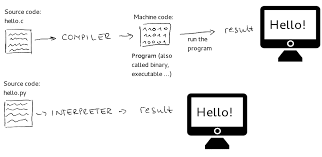
\includegraphics{index.png}
\caption{Interpreted vs compiled language}
\end{figure}

As a result, \(\tt{Python}\) is essentially an \emph{interactive}
programming language, you can program and see the results almost at the
same time. This is very nice in terms of readability of the code since
programmming is almost like instructing the computer in plain English
but it has drawbacks in term of perfomance since we have the
intermediate step of the ``translation'' (just to give an idea the
compilation of our C++ financial code takes more than one hour).

\begin{figure}
\centering
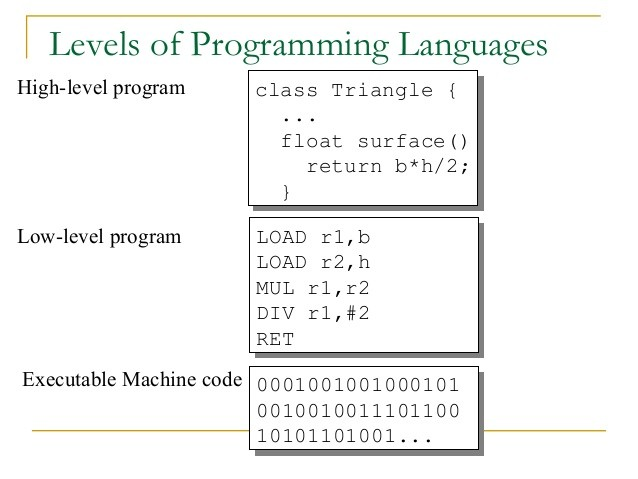
\includegraphics{machine_language.jpeg}
\caption{Human readable vs machine suitable code}
\end{figure}

\hypertarget{which-ttpython-should-i-use}{%
\subsubsection{\texorpdfstring{Which \(\tt{Python}\) should I use
?}{Which \textbackslash{}tt\{Python\} should I use ?}}\label{which-ttpython-should-i-use}}

\(\tt{Python}\), as basically all programs, comes in different version
and flavours as you can see by the number of updates the apps in your
mobile phone receives.

The latest version is \(\tt{3.8.5}\) (but it is continously evolving),
however you'll see older versions floating around (e.g.~\(\tt{2.7}\)).
This is because there are some big differences between
\(\tt{Python 2.X}\) and \(\tt{Python 3.X}\) which prevent a sizeable
portion of \(\tt{Python 2}\) users to stick with it since moving to
\(\tt{Python 3}\) would require a lot of work to adapt the code (this
process is usually called \emph{porting}).

\textbf{We will go for \(\tt{Python 3.7}\) !}

\hypertarget{how-can-i-use-ttpython}{%
\subsubsection{\texorpdfstring{How can I use \(\tt{Python}\)
?}{How can I use \textbackslash{}tt\{Python\} ?}}\label{how-can-i-use-ttpython}}

Once you have installed a \(\tt{Python}\) distribution there are various
ways of actually using it.

\begin{itemize}
\tightlist
\item
  the most immediate way is to just execute \(\tt{python.exe}\) on the
  command line to get a \(\tt{Python}\) console for interacting with the
  interpreter;
\item
  if you are learning \(\tt{Python}\) or do some simple data analysis,
  \$\tt{Jupyter notebooks} \$(i.e.~this document) allow to see the
  results of your code as you write it, as well as make notes, plot
  graphs beside it;
\item
  if you are a programmer and want to do more complex things, you'll
  usually want to split your code between more files to manage your
  project more easily. For this last case an integrated development
  environment (IDE) can be very useful. An IDE is a graphical user
  interface which makes writing complex code easier by providing a text
  editor, a file browser, a debugger (a tool that helps you to spot
  mistakes in your code) all in one software application. Good example
  is \(\tt{PyCharm}\) (https://www.jetbrains.com/pycharm/).
\end{itemize}

\hypertarget{online-courses}{%
\subsubsection{Online courses}\label{online-courses}}

\(\tt{Python}\) popularity is growing every day so it is very easy to
find good (and free) online courses looking into the web. Since in this
course we do not have time to cover in depth the potentiality of this
language I strongly suggest you to spend some time in watching one of
them. One example could be

\textbf{MITx: 6.00.1x Introduction to Computer Science and Programming
Using Python}
https://courses.edx.org/courses/course-v1:MITx+6.00.1x+2T2017\_2/course/

\hypertarget{python-basics}{%
\subsection{Python basics}\label{python-basics}}

Every language has \emph{keywords}, those are reserved words that have a
special meaning and tell the computer what to do. The first one we see
is \(\tt{print}\): it prints to screen whatever is specified between the
parenthesis.

    \begin{tcolorbox}[breakable, size=fbox, boxrule=1pt, pad at break*=1mm,colback=cellbackground, colframe=cellborder]
\prompt{In}{incolor}{1}{\boxspacing}
\begin{Verbatim}[commandchars=\\\{\}]
\PY{n+nb}{print} \PY{p}{(}\PY{l+s+s2}{\PYZdq{}}\PY{l+s+s2}{Hello world !}\PY{l+s+s2}{\PYZdq{}}\PY{p}{)} 
\end{Verbatim}
\end{tcolorbox}

    \begin{Verbatim}[commandchars=\\\{\}]
Hello world !
    \end{Verbatim}

    \begin{tcolorbox}[breakable, size=fbox, boxrule=1pt, pad at break*=1mm,colback=cellbackground, colframe=cellborder]
\prompt{In}{incolor}{2}{\boxspacing}
\begin{Verbatim}[commandchars=\\\{\}]
\PY{n+nb}{print} \PY{p}{(}\PY{l+s+s2}{\PYZdq{}}\PY{l+s+s2}{Welcome}\PY{l+s+s2}{\PYZdq{}}\PY{p}{)}
\PY{n+nb}{print} \PY{p}{(}\PY{l+s+s2}{\PYZdq{}}\PY{l+s+s2}{to}\PY{l+s+s2}{\PYZdq{}}\PY{p}{)}
\PY{n+nb}{print} \PY{p}{(}\PY{l+s+s2}{\PYZdq{}}\PY{l+s+s2}{everybody}\PY{l+s+s2}{\PYZdq{}}\PY{p}{)}
\end{Verbatim}
\end{tcolorbox}

    \begin{Verbatim}[commandchars=\\\{\}]
Welcome
to
everybody
    \end{Verbatim}

    Good programming practice recommends to document the code you write (it
is surprisingly easy to forget what you wanted to do in your code). In
\(\tt{python}\) you can add comments to the code starting your sentence
with a hash character (\#).

    \begin{tcolorbox}[breakable, size=fbox, boxrule=1pt, pad at break*=1mm,colback=cellbackground, colframe=cellborder]
\prompt{In}{incolor}{3}{\boxspacing}
\begin{Verbatim}[commandchars=\\\{\}]
\PY{c+c1}{\PYZsh{} this is a comment and the next line prints \PYZdq{}Ciao\PYZdq{}}
\PY{n+nb}{print} \PY{p}{(}\PY{l+s+s2}{\PYZdq{}}\PY{l+s+s2}{Ciao}\PY{l+s+s2}{\PYZdq{}}\PY{p}{)} \PY{c+c1}{\PYZsh{} comments like this are useful to explain what\PYZsq{}s going on in the }
               \PY{c+c1}{\PYZsh{} code you write}
\end{Verbatim}
\end{tcolorbox}

    \begin{Verbatim}[commandchars=\\\{\}]
Ciao
    \end{Verbatim}

    \hypertarget{variables}{%
\subsection{Variables}\label{variables}}

Variables are essentially labels you stick to some data (e.g.~a number,
a string\ldots{}). Variables and hence data they contain, can be used
referenced and manipulated throughout a program.

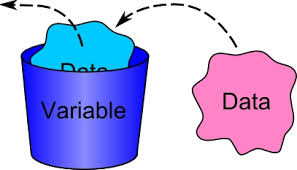
\includegraphics{var1.jpeg} 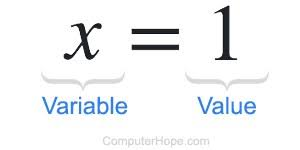
\includegraphics{var2.jpeg}

A variable can contain every kind of objects and is decleared using the
= operator. To inspect the content of a variable it can be used the
\(\tt{print}\) statement.

    \begin{tcolorbox}[breakable, size=fbox, boxrule=1pt, pad at break*=1mm,colback=cellbackground, colframe=cellborder]
\prompt{In}{incolor}{2}{\boxspacing}
\begin{Verbatim}[commandchars=\\\{\}]
\PY{n}{x} \PY{o}{=} \PY{l+m+mi}{9} \PY{c+c1}{\PYZsh{} assign number 9 to variable named x}
\PY{n+nb}{print} \PY{p}{(}\PY{n}{x}\PY{p}{)} 
\end{Verbatim}
\end{tcolorbox}

    \begin{Verbatim}[commandchars=\\\{\}]
9
    \end{Verbatim}

    \begin{tcolorbox}[breakable, size=fbox, boxrule=1pt, pad at break*=1mm,colback=cellbackground, colframe=cellborder]
\prompt{In}{incolor}{6}{\boxspacing}
\begin{Verbatim}[commandchars=\\\{\}]
\PY{n}{myphone} \PY{o}{=} \PY{l+s+s2}{\PYZdq{}}\PY{l+s+s2}{Huawei P10Lite}\PY{l+s+s2}{\PYZdq{}} \PY{c+c1}{\PYZsh{} in this case the variable contains a string}
\PY{n+nb}{print} \PY{p}{(}\PY{n}{myphone}\PY{p}{)}
\end{Verbatim}
\end{tcolorbox}

    Another very useful keyword is \(\tt{type}\), it tells which kind of
object is stored in a variable.

    \begin{tcolorbox}[breakable, size=fbox, boxrule=1pt, pad at break*=1mm,colback=cellbackground, colframe=cellborder]
\prompt{In}{incolor}{8}{\boxspacing}
\begin{Verbatim}[commandchars=\\\{\}]
\PY{n+nb}{print} \PY{p}{(}\PY{n+nb}{type}\PY{p}{(}\PY{n}{x}\PY{p}{)}\PY{p}{)}        
                      
\PY{n+nb}{print} \PY{p}{(}\PY{n+nb}{type}\PY{p}{(}\PY{n}{myphone}\PY{p}{)}\PY{p}{)} \PY{c+c1}{\PYZsh{} int\PYZhy{}\PYZgt{}integer, str\PYZhy{}\PYZgt{}string we will see later in more}
                      \PY{c+c1}{\PYZsh{} detail what is a string}
\end{Verbatim}
\end{tcolorbox}

    \begin{Verbatim}[commandchars=\\\{\}]
<class 'int'>
<class 'str'>
    \end{Verbatim}

    From now on I can use \(\tt{x}\) as an alias for a number or
\(\tt{myphone}\) as a string and manipuate their content for example I
can add 5 to \(\tt{x}\):

    \begin{tcolorbox}[breakable, size=fbox, boxrule=1pt, pad at break*=1mm,colback=cellbackground, colframe=cellborder]
\prompt{In}{incolor}{3}{\boxspacing}
\begin{Verbatim}[commandchars=\\\{\}]
\PY{n+nb}{print} \PY{p}{(}\PY{n}{x}\PY{o}{+}\PY{l+m+mi}{5}\PY{p}{)}
\end{Verbatim}
\end{tcolorbox}

    \begin{Verbatim}[commandchars=\\\{\}]
14
    \end{Verbatim}

    \hypertarget{variable-name-rules}{%
\subsubsection{Variable name rules}\label{variable-name-rules}}

A \(\tt{python}\) variable name must: * begin with a letter (myphone) or
underscore (\_myphone); * other characters can be letters, numbers or
more \_; * variable names are case-sensitive so myphone and myPhone are
two distinct variables.

\textbf{Keywords are reserved words as such you cannot use as variable
names (e.g.~\(\tt{print, type, for...}\))}.

To use GOOD variable names always choose meaningful names instead of
short names (i.e.~\(\tt{numberOfCakes}\) is much better than simply
\(\tt{n}\)), try to be consistent with your conventions (e.g.~choose
once and for all between \(\tt{number\_of\_cakes}\) or
\(\tt{numberofcakes}\) or \(\tt{numberOfCakes}\)), usually begin a
variable name with underscore (\_) only for a special case (will see
later when this is usually done).

\hypertarget{mathematical-expressions}{%
\subsection{Mathematical expressions}\label{mathematical-expressions}}

    \begin{tcolorbox}[breakable, size=fbox, boxrule=1pt, pad at break*=1mm,colback=cellbackground, colframe=cellborder]
\prompt{In}{incolor}{9}{\boxspacing}
\begin{Verbatim}[commandchars=\\\{\}]
\PY{l+m+mi}{1} \PY{o}{+} \PY{l+m+mi}{2}
\end{Verbatim}
\end{tcolorbox}

            \begin{tcolorbox}[breakable, size=fbox, boxrule=.5pt, pad at break*=1mm, opacityfill=0]
\prompt{Out}{outcolor}{9}{\boxspacing}
\begin{Verbatim}[commandchars=\\\{\}]
3
\end{Verbatim}
\end{tcolorbox}
        
    \begin{tcolorbox}[breakable, size=fbox, boxrule=1pt, pad at break*=1mm,colback=cellbackground, colframe=cellborder]
\prompt{In}{incolor}{10}{\boxspacing}
\begin{Verbatim}[commandchars=\\\{\}]
\PY{l+m+mi}{40} \PY{o}{\PYZhy{}} \PY{l+m+mi}{5}
\end{Verbatim}
\end{tcolorbox}

            \begin{tcolorbox}[breakable, size=fbox, boxrule=.5pt, pad at break*=1mm, opacityfill=0]
\prompt{Out}{outcolor}{10}{\boxspacing}
\begin{Verbatim}[commandchars=\\\{\}]
35
\end{Verbatim}
\end{tcolorbox}
        
    \begin{tcolorbox}[breakable, size=fbox, boxrule=1pt, pad at break*=1mm,colback=cellbackground, colframe=cellborder]
\prompt{In}{incolor}{11}{\boxspacing}
\begin{Verbatim}[commandchars=\\\{\}]
\PY{n}{x} \PY{o}{*} \PY{l+m+mi}{20} \PY{c+c1}{\PYZsh{} remember that we set x equal to 9}
\end{Verbatim}
\end{tcolorbox}

            \begin{tcolorbox}[breakable, size=fbox, boxrule=.5pt, pad at break*=1mm, opacityfill=0]
\prompt{Out}{outcolor}{11}{\boxspacing}
\begin{Verbatim}[commandchars=\\\{\}]
180
\end{Verbatim}
\end{tcolorbox}
        
    \begin{tcolorbox}[breakable, size=fbox, boxrule=1pt, pad at break*=1mm,colback=cellbackground, colframe=cellborder]
\prompt{In}{incolor}{12}{\boxspacing}
\begin{Verbatim}[commandchars=\\\{\}]
\PY{n}{x} \PY{o}{/} \PY{l+m+mi}{4}
\end{Verbatim}
\end{tcolorbox}

            \begin{tcolorbox}[breakable, size=fbox, boxrule=.5pt, pad at break*=1mm, opacityfill=0]
\prompt{Out}{outcolor}{12}{\boxspacing}
\begin{Verbatim}[commandchars=\\\{\}]
2.25
\end{Verbatim}
\end{tcolorbox}
        
    \begin{tcolorbox}[breakable, size=fbox, boxrule=1pt, pad at break*=1mm,colback=cellbackground, colframe=cellborder]
\prompt{In}{incolor}{13}{\boxspacing}
\begin{Verbatim}[commandchars=\\\{\}]
\PY{n+nb}{print} \PY{p}{(}\PY{n+nb}{type}\PY{p}{(}\PY{l+m+mf}{2.25}\PY{p}{)}\PY{p}{)} \PY{c+c1}{\PYZsh{} this is a new type: floating\PYZhy{}point value}
\end{Verbatim}
\end{tcolorbox}

    \begin{Verbatim}[commandchars=\\\{\}]
<class 'float'>
    \end{Verbatim}

    \begin{tcolorbox}[breakable, size=fbox, boxrule=1pt, pad at break*=1mm,colback=cellbackground, colframe=cellborder]
\prompt{In}{incolor}{14}{\boxspacing}
\begin{Verbatim}[commandchars=\\\{\}]
\PY{n}{x} \PY{o}{/}\PY{o}{/} \PY{l+m+mi}{4} \PY{c+c1}{\PYZsh{} interger division \PYZhy{} result will be truncated to the }
       \PY{c+c1}{\PYZsh{} corresponding integer (no rounding)}
       \PY{c+c1}{\PYZsh{} 11 / 3 = 3.666666 \PYZhy{}\PYZgt{} 11 // 3 = 3}
\end{Verbatim}
\end{tcolorbox}

            \begin{tcolorbox}[breakable, size=fbox, boxrule=.5pt, pad at break*=1mm, opacityfill=0]
\prompt{Out}{outcolor}{14}{\boxspacing}
\begin{Verbatim}[commandchars=\\\{\}]
2
\end{Verbatim}
\end{tcolorbox}
        
    \begin{tcolorbox}[breakable, size=fbox, boxrule=1pt, pad at break*=1mm,colback=cellbackground, colframe=cellborder]
\prompt{In}{incolor}{15}{\boxspacing}
\begin{Verbatim}[commandchars=\\\{\}]
\PY{n}{y} \PY{o}{=} \PY{l+m+mi}{3}
\PY{n}{x} \PY{o}{*}\PY{o}{*} \PY{n}{y} \PY{c+c1}{\PYZsh{} x to the power of y}
\end{Verbatim}
\end{tcolorbox}

            \begin{tcolorbox}[breakable, size=fbox, boxrule=.5pt, pad at break*=1mm, opacityfill=0]
\prompt{Out}{outcolor}{15}{\boxspacing}
\begin{Verbatim}[commandchars=\\\{\}]
729
\end{Verbatim}
\end{tcolorbox}
        
    \begin{tcolorbox}[breakable, size=fbox, boxrule=1pt, pad at break*=1mm,colback=cellbackground, colframe=cellborder]
\prompt{In}{incolor}{16}{\boxspacing}
\begin{Verbatim}[commandchars=\\\{\}]
\PY{l+m+mi}{3} \PY{o}{*} \PY{p}{(}\PY{n}{x} \PY{o}{+} \PY{n}{y}\PY{p}{)}
\end{Verbatim}
\end{tcolorbox}

            \begin{tcolorbox}[breakable, size=fbox, boxrule=.5pt, pad at break*=1mm, opacityfill=0]
\prompt{Out}{outcolor}{16}{\boxspacing}
\begin{Verbatim}[commandchars=\\\{\}]
36
\end{Verbatim}
\end{tcolorbox}
        
    As an example of variable manipulation let's try to increment \(\tt{x}\)
by 1 and save the result again in \(\tt{x}\).

    \begin{tcolorbox}[breakable, size=fbox, boxrule=1pt, pad at break*=1mm,colback=cellbackground, colframe=cellborder]
\prompt{In}{incolor}{12}{\boxspacing}
\begin{Verbatim}[commandchars=\\\{\}]
\PY{n+nb}{print} \PY{p}{(}\PY{n}{x}\PY{p}{)}
\PY{n}{x} \PY{o}{=} \PY{n}{x} \PY{o}{+} \PY{l+m+mi}{1}
\PY{n+nb}{print} \PY{p}{(}\PY{n}{x}\PY{p}{)}
\end{Verbatim}
\end{tcolorbox}

    \begin{Verbatim}[commandchars=\\\{\}]
15
16
    \end{Verbatim}

    More complex mathematical functions are not directly available, let's
see for example the logarithm:

    \begin{tcolorbox}[breakable, size=fbox, boxrule=1pt, pad at break*=1mm,colback=cellbackground, colframe=cellborder]
\prompt{In}{incolor}{17}{\boxspacing}
\begin{Verbatim}[commandchars=\\\{\}]
\PY{n}{log}\PY{p}{(}\PY{l+m+mi}{3}\PY{p}{)}
\end{Verbatim}
\end{tcolorbox}

    \begin{Verbatim}[commandchars=\\\{\}]

        ---------------------------------------------------------------------------

        NameError                                 Traceback (most recent call last)

        <ipython-input-17-ffde4d60496a> in <module>()
    ----> 1 log(3) \# causes an error because the logarithm function
          2        \# is not available by default


        NameError: name 'log' is not defined

    \end{Verbatim}

    \hypertarget{modules}{%
\subsection{Modules}\label{modules}}

One very important feature of each language is the ability to reuse code
in different programs, e.g.~imagine how awful would be if you had to
reimplement every time you need it a function to compute the logarithm.
Usually there are mechanisms that allow to collect useful routines in
\emph{packages} (or \emph{libraries}, or \emph{modules}) so that later
they can be called and used by any program may need them.

These collections of utilities in \(\tt{python}\) are called
\emph{modules} and every time you install it, it comes with a standard
set of them. If you need more functionality, you can download more of
them (there are zillions of packages out there) or you can of course
write your own (which is the goal of this course in the end).

Some examples of useful modules we will use are:

\begin{itemize}
\tightlist
\item
  Numpy - which provides matrix algebra functionality and much more;
\item
  Scipy - which provides a whole series of scientific computing
  functions;
\item
  Pandas - which provides tools for manipulating time series or dataset
  in general;
\item
  Matplotlib - for plotting graphs;
\item
  Jupyter - for notebooks like this one.
\end{itemize}

\begin{figure}
\centering
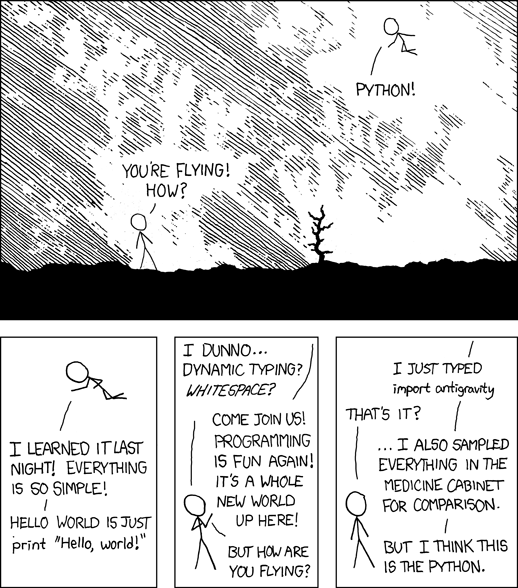
\includegraphics{python.png}
\caption{Python has many modules for download on the web\ldots{}}
\end{figure}

In order to load a module in a \(\tt{python}\) program you can use the
\(\tt{import}\) keyword. Information on a module can be retrieved using
\(\tt{help}\) and \(\tt{dir}\) keywords: the first write a help message
which usually describes the functionalities of a module, the latter list
all the available functions of a module. \textbf{In order to access a
function of a module you have to use the . (dot) operator:
module\_name.function.} Let's see an example dealing with the
\(\tt{math}\) module which implements the most common mathematical
functions.

    \begin{tcolorbox}[breakable, size=fbox, boxrule=1pt, pad at break*=1mm,colback=cellbackground, colframe=cellborder]
\prompt{In}{incolor}{4}{\boxspacing}
\begin{Verbatim}[commandchars=\\\{\}]
\PY{k+kn}{import} \PY{n+nn}{math} \PY{c+c1}{\PYZsh{} make available the math module}
\PY{n+nb}{dir}\PY{p}{(}\PY{n}{math}\PY{p}{)} \PY{c+c1}{\PYZsh{} list its content}
\end{Verbatim}
\end{tcolorbox}

            \begin{tcolorbox}[breakable, size=fbox, boxrule=.5pt, pad at break*=1mm, opacityfill=0]
\prompt{Out}{outcolor}{4}{\boxspacing}
\begin{Verbatim}[commandchars=\\\{\}]
['\_\_doc\_\_',
 '\_\_file\_\_',
 '\_\_loader\_\_',
 '\_\_name\_\_',
 '\_\_package\_\_',
 '\_\_spec\_\_',
 'acos',
 'acosh',
 'asin',
 'asinh',
 'atan',
 'atan2',
 'atanh',
 'ceil',
 'copysign',
 'cos',
 'cosh',
 'degrees',
 'e',
 'erf',
 'erfc',
 'exp',
 'expm1',
 'fabs',
 'factorial',
 'floor',
 'fmod',
 'frexp',
 'fsum',
 'gamma',
 'gcd',
 'hypot',
 'inf',
 'isclose',
 'isfinite',
 'isinf',
 'isnan',
 'ldexp',
 'lgamma',
 'log',
 'log10',
 'log1p',
 'log2',
 'modf',
 'nan',
 'pi',
 'pow',
 'radians',
 'sin',
 'sinh',
 'sqrt',
 'tan',
 'tanh',
 'tau',
 'trunc']
\end{Verbatim}
\end{tcolorbox}
        
    \begin{tcolorbox}[breakable, size=fbox, boxrule=1pt, pad at break*=1mm,colback=cellbackground, colframe=cellborder]
\prompt{In}{incolor}{5}{\boxspacing}
\begin{Verbatim}[commandchars=\\\{\}]
\PY{n}{help}\PY{p}{(}\PY{n}{math}\PY{p}{)}
\end{Verbatim}
\end{tcolorbox}

    \begin{Verbatim}[commandchars=\\\{\}]
Help on module math:

NAME
    math

MODULE REFERENCE
    https://docs.python.org/3.6/library/math

    The following documentation is automatically generated from the Python
    source files.  It may be incomplete, incorrect or include features that
    are considered implementation detail and may vary between Python
    implementations.  When in doubt, consult the module reference at the
    location listed above.

DESCRIPTION
    This module is always available.  It provides access to the
    mathematical functions defined by the C standard.

FUNCTIONS
    acos({\ldots})
        acos(x)

        Return the arc cosine (measured in radians) of x.

    acosh({\ldots})
        acosh(x)

        Return the inverse hyperbolic cosine of x.

    asin({\ldots})
        asin(x)

        Return the arc sine (measured in radians) of x.

    asinh({\ldots})
        asinh(x)

        Return the inverse hyperbolic sine of x.

    atan({\ldots})
        atan(x)

        Return the arc tangent (measured in radians) of x.

    atan2({\ldots})
        atan2(y, x)

        Return the arc tangent (measured in radians) of y/x.
        Unlike atan(y/x), the signs of both x and y are considered.

    atanh({\ldots})
        atanh(x)

        Return the inverse hyperbolic tangent of x.

    ceil({\ldots})
        ceil(x)

        Return the ceiling of x as an Integral.
        This is the smallest integer >= x.

    copysign({\ldots})
        copysign(x, y)

        Return a float with the magnitude (absolute value) of x but the sign
        of y. On platforms that support signed zeros, copysign(1.0, -0.0)
        returns -1.0.

    cos({\ldots})
        cos(x)

        Return the cosine of x (measured in radians).

    cosh({\ldots})
        cosh(x)

        Return the hyperbolic cosine of x.

    degrees({\ldots})
        degrees(x)

        Convert angle x from radians to degrees.

    erf({\ldots})
        erf(x)

        Error function at x.

    erfc({\ldots})
        erfc(x)

        Complementary error function at x.

    exp({\ldots})
        exp(x)

        Return e raised to the power of x.

    expm1({\ldots})
        expm1(x)

        Return exp(x)-1.
        This function avoids the loss of precision involved in the direct
evaluation of exp(x)-1 for small x.

    fabs({\ldots})
        fabs(x)

        Return the absolute value of the float x.

    factorial({\ldots})
        factorial(x) -> Integral

        Find x!. Raise a ValueError if x is negative or non-integral.

    floor({\ldots})
        floor(x)

        Return the floor of x as an Integral.
        This is the largest integer <= x.

    fmod({\ldots})
        fmod(x, y)

        Return fmod(x, y), according to platform C.  x \% y may differ.

    frexp({\ldots})
        frexp(x)

        Return the mantissa and exponent of x, as pair (m, e).
        m is a float and e is an int, such that x = m * 2.**e.
        If x is 0, m and e are both 0.  Else 0.5 <= abs(m) < 1.0.

    fsum({\ldots})
        fsum(iterable)

        Return an accurate floating point sum of values in the iterable.
        Assumes IEEE-754 floating point arithmetic.

    gamma({\ldots})
        gamma(x)

        Gamma function at x.

    gcd({\ldots})
        gcd(x, y) -> int
        greatest common divisor of x and y

    hypot({\ldots})
        hypot(x, y)

        Return the Euclidean distance, sqrt(x*x + y*y).

    isclose({\ldots})
        isclose(a, b, *, rel\_tol=1e-09, abs\_tol=0.0) -> bool

        Determine whether two floating point numbers are close in value.

           rel\_tol
               maximum difference for being considered "close", relative to the
               magnitude of the input values
            abs\_tol
               maximum difference for being considered "close", regardless of
the
               magnitude of the input values

        Return True if a is close in value to b, and False otherwise.

        For the values to be considered close, the difference between them
        must be smaller than at least one of the tolerances.

        -inf, inf and NaN behave similarly to the IEEE 754 Standard.  That
        is, NaN is not close to anything, even itself.  inf and -inf are
        only close to themselves.

    isfinite({\ldots})
        isfinite(x) -> bool

        Return True if x is neither an infinity nor a NaN, and False otherwise.

    isinf({\ldots})
        isinf(x) -> bool

        Return True if x is a positive or negative infinity, and False
otherwise.

    isnan({\ldots})
        isnan(x) -> bool

        Return True if x is a NaN (not a number), and False otherwise.

    ldexp({\ldots})
        ldexp(x, i)

        Return x * (2**i).

    lgamma({\ldots})
        lgamma(x)

        Natural logarithm of absolute value of Gamma function at x.

    log({\ldots})
        log(x[, base])

        Return the logarithm of x to the given base.
        If the base not specified, returns the natural logarithm (base e) of x.

    log10({\ldots})
        log10(x)

        Return the base 10 logarithm of x.

    log1p({\ldots})
        log1p(x)

        Return the natural logarithm of 1+x (base e).
        The result is computed in a way which is accurate for x near zero.

    log2({\ldots})
        log2(x)

        Return the base 2 logarithm of x.

    modf({\ldots})
        modf(x)

        Return the fractional and integer parts of x.  Both results carry the
sign
        of x and are floats.

    pow({\ldots})
        pow(x, y)

        Return x**y (x to the power of y).

    radians({\ldots})
        radians(x)

        Convert angle x from degrees to radians.

    sin({\ldots})
        sin(x)

        Return the sine of x (measured in radians).

    sinh({\ldots})
        sinh(x)

        Return the hyperbolic sine of x.

    sqrt({\ldots})
        sqrt(x)

        Return the square root of x.

    tan({\ldots})
        tan(x)

        Return the tangent of x (measured in radians).

    tanh({\ldots})
        tanh(x)

        Return the hyperbolic tangent of x.

    trunc({\ldots})
        trunc(x:Real) -> Integral

        Truncates x to the nearest Integral toward 0. Uses the \_\_trunc\_\_ magic
method.

DATA
    e = 2.718281828459045
    inf = inf
    nan = nan
    pi = 3.141592653589793
    tau = 6.283185307179586

FILE
    /home/sani/anaconda3/envs/.python3/lib/python3.6/lib-
dynload/math.cpython-36m-x86\_64-linux-gnu.so


    \end{Verbatim}

    \begin{tcolorbox}[breakable, size=fbox, boxrule=1pt, pad at break*=1mm,colback=cellbackground, colframe=cellborder]
\prompt{In}{incolor}{19}{\boxspacing}
\begin{Verbatim}[commandchars=\\\{\}]
\PY{n}{math}\PY{o}{.}\PY{n}{log}\PY{p}{(}\PY{l+m+mi}{3}\PY{p}{)} \PY{c+c1}{\PYZsh{} accessing the logarithm function}
\end{Verbatim}
\end{tcolorbox}

            \begin{tcolorbox}[breakable, size=fbox, boxrule=.5pt, pad at break*=1mm, opacityfill=0]
\prompt{Out}{outcolor}{19}{\boxspacing}
\begin{Verbatim}[commandchars=\\\{\}]
1.0986122886681098
\end{Verbatim}
\end{tcolorbox}
        
    \begin{tcolorbox}[breakable, size=fbox, boxrule=1pt, pad at break*=1mm,colback=cellbackground, colframe=cellborder]
\prompt{In}{incolor}{20}{\boxspacing}
\begin{Verbatim}[commandchars=\\\{\}]
\PY{n}{math}\PY{o}{.}\PY{n}{exp}\PY{p}{(}\PY{l+m+mi}{3}\PY{p}{)} \PY{c+c1}{\PYZsh{} accessing the exponential function}
\end{Verbatim}
\end{tcolorbox}

            \begin{tcolorbox}[breakable, size=fbox, boxrule=.5pt, pad at break*=1mm, opacityfill=0]
\prompt{Out}{outcolor}{20}{\boxspacing}
\begin{Verbatim}[commandchars=\\\{\}]
20.085536923187668
\end{Verbatim}
\end{tcolorbox}
        
    \begin{tcolorbox}[breakable, size=fbox, boxrule=1pt, pad at break*=1mm,colback=cellbackground, colframe=cellborder]
\prompt{In}{incolor}{21}{\boxspacing}
\begin{Verbatim}[commandchars=\\\{\}]
\PY{n+nb}{print} \PY{p}{(}\PY{n+nb}{type}\PY{p}{(}\PY{n}{math}\PY{o}{.}\PY{n}{log}\PY{p}{)}\PY{p}{)} \PY{c+c1}{\PYZsh{} yet another type: builtin function}
\PY{n+nb}{print} \PY{p}{(}\PY{n+nb}{type}\PY{p}{(}\PY{n}{math}\PY{o}{.}\PY{n}{log}\PY{p}{(}\PY{l+m+mi}{3}\PY{p}{)}\PY{p}{)}\PY{p}{)}
\end{Verbatim}
\end{tcolorbox}

    \begin{Verbatim}[commandchars=\\\{\}]
<class 'builtin\_function\_or\_method'>
<class 'float'>
    \end{Verbatim}

    Since we are lazy and we don't want to type ``math.'' every time we
compute a logarithm or an exponential, we can just import the needed
functions from a module using the following syntax:

    \begin{tcolorbox}[breakable, size=fbox, boxrule=1pt, pad at break*=1mm,colback=cellbackground, colframe=cellborder]
\prompt{In}{incolor}{7}{\boxspacing}
\begin{Verbatim}[commandchars=\\\{\}]
\PY{k+kn}{from} \PY{n+nn}{math} \PY{k}{import} \PY{n}{log}\PY{p}{,} \PY{n}{exp}
\PY{n+nb}{print} \PY{p}{(}\PY{n}{log}\PY{p}{(}\PY{l+m+mi}{3}\PY{p}{)}\PY{p}{)}
\PY{n+nb}{print} \PY{p}{(}\PY{n}{exp}\PY{p}{(}\PY{l+m+mi}{3}\PY{p}{)}\PY{p}{)}
\end{Verbatim}
\end{tcolorbox}

    \begin{Verbatim}[commandchars=\\\{\}]
1.0986122886681098
20.085536923187668
    \end{Verbatim}

    As an example let's compute the interest rate \(r\) that produces a
return \(R\) of about 11000 Euro when investing 10000 Euro for 2 years:

\(R = N\mathrm{e}^{r\tau} \rightarrow r = \frac{1}{\tau} \mathrm{log}(\frac{R}{N})\)

    \begin{tcolorbox}[breakable, size=fbox, boxrule=1pt, pad at break*=1mm,colback=cellbackground, colframe=cellborder]
\prompt{In}{incolor}{11}{\boxspacing}
\begin{Verbatim}[commandchars=\\\{\}]
\PY{n}{rate} \PY{o}{=} \PY{p}{(}\PY{l+m+mi}{1}\PY{o}{/}\PY{l+m+mi}{2}\PY{p}{)}\PY{o}{*}\PY{n}{log}\PY{p}{(}\PY{l+m+mi}{11000}\PY{o}{/}\PY{l+m+mi}{10000}\PY{p}{)}
\PY{n+nb}{print} \PY{p}{(}\PY{n}{rate}\PY{p}{)}
\end{Verbatim}
\end{tcolorbox}

    \begin{Verbatim}[commandchars=\\\{\}]
0.04765508990216247
    \end{Verbatim}

    \hypertarget{boolean-expressions}{%
\subsection{Boolean expressions}\label{boolean-expressions}}

The expressions we have seen so far evaluate to a number. Boolean
expressions evaluate to \(\tt{true}\) or \(\tt{false}\) only. This type
of expressions usually involve logical or comparison operators like
\(\tt{or}\), \(\tt{and}\), \textgreater{} (greater than), \textless{}
(less than)\ldots{} Let's see some example. The following expression
answer the question is 1 equal to 2:

    \begin{tcolorbox}[breakable, size=fbox, boxrule=1pt, pad at break*=1mm,colback=cellbackground, colframe=cellborder]
\prompt{In}{incolor}{24}{\boxspacing}
\begin{Verbatim}[commandchars=\\\{\}]
\PY{l+m+mi}{1} \PY{o}{==} \PY{l+m+mi}{2} 
\PY{c+c1}{\PYZsh{} single = assigns a value to a variable like in x = 9}
\PY{c+c1}{\PYZsh{} double == checks the equality of two objects}
\end{Verbatim}
\end{tcolorbox}

            \begin{tcolorbox}[breakable, size=fbox, boxrule=.5pt, pad at break*=1mm, opacityfill=0]
\prompt{Out}{outcolor}{24}{\boxspacing}
\begin{Verbatim}[commandchars=\\\{\}]
False
\end{Verbatim}
\end{tcolorbox}
        
    \begin{tcolorbox}[breakable, size=fbox, boxrule=1pt, pad at break*=1mm,colback=cellbackground, colframe=cellborder]
\prompt{In}{incolor}{25}{\boxspacing}
\begin{Verbatim}[commandchars=\\\{\}]
\PY{l+m+mi}{1} \PY{o}{!=} \PY{l+m+mi}{2} \PY{c+c1}{\PYZsh{} != is the \PYZdq{}not equal to\PYZdq{} operator}
\end{Verbatim}
\end{tcolorbox}

            \begin{tcolorbox}[breakable, size=fbox, boxrule=.5pt, pad at break*=1mm, opacityfill=0]
\prompt{Out}{outcolor}{25}{\boxspacing}
\begin{Verbatim}[commandchars=\\\{\}]
True
\end{Verbatim}
\end{tcolorbox}
        
    \begin{tcolorbox}[breakable, size=fbox, boxrule=1pt, pad at break*=1mm,colback=cellbackground, colframe=cellborder]
\prompt{In}{incolor}{26}{\boxspacing}
\begin{Verbatim}[commandchars=\\\{\}]
\PY{l+m+mi}{2} \PY{o}{\PYZlt{}} \PY{l+m+mi}{2}
\end{Verbatim}
\end{tcolorbox}

            \begin{tcolorbox}[breakable, size=fbox, boxrule=.5pt, pad at break*=1mm, opacityfill=0]
\prompt{Out}{outcolor}{26}{\boxspacing}
\begin{Verbatim}[commandchars=\\\{\}]
False
\end{Verbatim}
\end{tcolorbox}
        
    \begin{tcolorbox}[breakable, size=fbox, boxrule=1pt, pad at break*=1mm,colback=cellbackground, colframe=cellborder]
\prompt{In}{incolor}{27}{\boxspacing}
\begin{Verbatim}[commandchars=\\\{\}]
\PY{l+m+mi}{2} \PY{o}{\PYZlt{}}\PY{o}{=} \PY{l+m+mi}{2}  \PY{c+c1}{\PYZsh{} in this case we allow the numbers to be equal too}
\end{Verbatim}
\end{tcolorbox}

            \begin{tcolorbox}[breakable, size=fbox, boxrule=.5pt, pad at break*=1mm, opacityfill=0]
\prompt{Out}{outcolor}{27}{\boxspacing}
\begin{Verbatim}[commandchars=\\\{\}]
True
\end{Verbatim}
\end{tcolorbox}
        
    \begin{tcolorbox}[breakable, size=fbox, boxrule=1pt, pad at break*=1mm,colback=cellbackground, colframe=cellborder]
\prompt{In}{incolor}{28}{\boxspacing}
\begin{Verbatim}[commandchars=\\\{\}]
\PY{n+nb}{print} \PY{p}{(}\PY{n}{x}\PY{p}{)}
\PY{l+m+mi}{15} \PY{o}{\PYZlt{}}\PY{o}{=} \PY{n}{x} \PY{o+ow}{and} \PY{n}{x} \PY{o}{\PYZlt{}}\PY{o}{=} \PY{l+m+mi}{20} 
\end{Verbatim}
\end{tcolorbox}

    \begin{Verbatim}[commandchars=\\\{\}]
11
    \end{Verbatim}

            \begin{tcolorbox}[breakable, size=fbox, boxrule=.5pt, pad at break*=1mm, opacityfill=0]
\prompt{Out}{outcolor}{28}{\boxspacing}
\begin{Verbatim}[commandchars=\\\{\}]
False
\end{Verbatim}
\end{tcolorbox}
        
    \begin{tcolorbox}[breakable, size=fbox, boxrule=1pt, pad at break*=1mm,colback=cellbackground, colframe=cellborder]
\prompt{In}{incolor}{29}{\boxspacing}
\begin{Verbatim}[commandchars=\\\{\}]
\PY{l+m+mi}{15} \PY{o}{\PYZlt{}}\PY{o}{=} \PY{n}{x} \PY{o+ow}{or} \PY{n}{x} \PY{o}{\PYZlt{}}\PY{o}{=} \PY{l+m+mi}{20}
\end{Verbatim}
\end{tcolorbox}

            \begin{tcolorbox}[breakable, size=fbox, boxrule=.5pt, pad at break*=1mm, opacityfill=0]
\prompt{Out}{outcolor}{29}{\boxspacing}
\begin{Verbatim}[commandchars=\\\{\}]
True
\end{Verbatim}
\end{tcolorbox}
        
    \begin{tcolorbox}[breakable, size=fbox, boxrule=1pt, pad at break*=1mm,colback=cellbackground, colframe=cellborder]
\prompt{In}{incolor}{30}{\boxspacing}
\begin{Verbatim}[commandchars=\\\{\}]
\PY{o+ow}{not} \PY{p}{(}\PY{n}{x} \PY{o}{\PYZgt{}} \PY{l+m+mi}{20}\PY{p}{)} \PY{c+c1}{\PYZsh{} the not keyword negates the following expression}
\end{Verbatim}
\end{tcolorbox}

            \begin{tcolorbox}[breakable, size=fbox, boxrule=.5pt, pad at break*=1mm, opacityfill=0]
\prompt{Out}{outcolor}{30}{\boxspacing}
\begin{Verbatim}[commandchars=\\\{\}]
True
\end{Verbatim}
\end{tcolorbox}
        
    \hypertarget{string-expressions}{%
\subsection{String expressions}\label{string-expressions}}

A ``string'' is a sequence of characters (letters, digits, spaces,
punctuation, new lines\ldots{}). There are many operations that can be
performed on strings, like concatenate (with + operator), truncate,
replace\ldots{}

    \begin{tcolorbox}[breakable, size=fbox, boxrule=1pt, pad at break*=1mm,colback=cellbackground, colframe=cellborder]
\prompt{In}{incolor}{14}{\boxspacing}
\begin{Verbatim}[commandchars=\\\{\}]
\PY{n}{mystring} \PY{o}{=} \PY{l+s+s2}{\PYZdq{}}\PY{l+s+s2}{some text with punctuation, spaces and digits 10}\PY{l+s+s2}{\PYZdq{}}
\end{Verbatim}
\end{tcolorbox}

    \begin{tcolorbox}[breakable, size=fbox, boxrule=1pt, pad at break*=1mm,colback=cellbackground, colframe=cellborder]
\prompt{In}{incolor}{16}{\boxspacing}
\begin{Verbatim}[commandchars=\\\{\}]
\PY{n}{mystring}\PY{o}{.}\PY{n}{replace}\PY{p}{(}\PY{l+s+s2}{\PYZdq{}}\PY{l+s+s2}{s}\PY{l+s+s2}{\PYZdq{}}\PY{p}{,} \PY{l+s+s2}{\PYZdq{}}\PY{l+s+s2}{z}\PY{l+s+s2}{\PYZdq{}}\PY{p}{)}
\end{Verbatim}
\end{tcolorbox}

            \begin{tcolorbox}[breakable, size=fbox, boxrule=.5pt, pad at break*=1mm, opacityfill=0]
\prompt{Out}{outcolor}{16}{\boxspacing}
\begin{Verbatim}[commandchars=\\\{\}]
'zome text with punctuation, zpacez and digitz 10'
\end{Verbatim}
\end{tcolorbox}
        
    \begin{tcolorbox}[breakable, size=fbox, boxrule=1pt, pad at break*=1mm,colback=cellbackground, colframe=cellborder]
\prompt{In}{incolor}{15}{\boxspacing}
\begin{Verbatim}[commandchars=\\\{\}]
\PY{l+s+s2}{\PYZdq{}}\PY{l+s+s2}{abc}\PY{l+s+s2}{\PYZdq{}} \PY{o}{+} \PY{l+s+s2}{\PYZdq{}}\PY{l+s+s2}{def}\PY{l+s+s2}{\PYZdq{}}  
\end{Verbatim}
\end{tcolorbox}

            \begin{tcolorbox}[breakable, size=fbox, boxrule=.5pt, pad at break*=1mm, opacityfill=0]
\prompt{Out}{outcolor}{15}{\boxspacing}
\begin{Verbatim}[commandchars=\\\{\}]
'abcdef'
\end{Verbatim}
\end{tcolorbox}
        
    \begin{tcolorbox}[breakable, size=fbox, boxrule=1pt, pad at break*=1mm,colback=cellbackground, colframe=cellborder]
\prompt{In}{incolor}{33}{\boxspacing}
\begin{Verbatim}[commandchars=\\\{\}]
\PY{l+s+s2}{\PYZdq{}}\PY{l+s+s2}{The number }\PY{l+s+s2}{\PYZdq{}} \PY{o}{+} \PY{l+m+mi}{4} \PY{o}{+} \PY{l+s+s2}{\PYZdq{}}\PY{l+s+s2}{ is my favourite number}\PY{l+s+s2}{\PYZdq{}}
\PY{c+c1}{\PYZsh{} this causes an error since we are trying to concatenate a string }
\PY{c+c1}{\PYZsh{} with a number so two different kind of objects}
\end{Verbatim}
\end{tcolorbox}

    \begin{Verbatim}[commandchars=\\\{\}]

        ---------------------------------------------------------------------------

        TypeError                                 Traceback (most recent call last)

        <ipython-input-33-b9f65c5a45f7> in <module>()
    ----> 1 "The number " + 4 + " is my favourite number"
          2 \# this causes an error since we are trying to concatenate a string
          3 \# with a number so two different kind of objects


        TypeError: can only concatenate str (not "int") to str

    \end{Verbatim}

    To avoid this error is possible to \textbf{cast} an object to a
different type, \(\tt{python}\) will try then to convert it to the
desired type. In this case we can \emph{force} the number four to be
represented as a string with the \(\tt{str()}\) function:

    \begin{tcolorbox}[breakable, size=fbox, boxrule=1pt, pad at break*=1mm,colback=cellbackground, colframe=cellborder]
\prompt{In}{incolor}{34}{\boxspacing}
\begin{Verbatim}[commandchars=\\\{\}]
\PY{l+s+s2}{\PYZdq{}}\PY{l+s+s2}{The number }\PY{l+s+s2}{\PYZdq{}} \PY{o}{+} \PY{n+nb}{str}\PY{p}{(}\PY{l+m+mi}{4}\PY{p}{)} \PY{o}{+} \PY{l+s+s2}{\PYZdq{}}\PY{l+s+s2}{ is my favourite number}\PY{l+s+s2}{\PYZdq{}}
\end{Verbatim}
\end{tcolorbox}

            \begin{tcolorbox}[breakable, size=fbox, boxrule=.5pt, pad at break*=1mm, opacityfill=0]
\prompt{Out}{outcolor}{34}{\boxspacing}
\begin{Verbatim}[commandchars=\\\{\}]
'The number 4 is my favourite number'
\end{Verbatim}
\end{tcolorbox}
        
    \begin{tcolorbox}[breakable, size=fbox, boxrule=1pt, pad at break*=1mm,colback=cellbackground, colframe=cellborder]
\prompt{In}{incolor}{35}{\boxspacing}
\begin{Verbatim}[commandchars=\\\{\}]
\PY{n+nb}{print} \PY{p}{(}\PY{n+nb}{type}\PY{p}{(}\PY{l+m+mf}{3.4}\PY{p}{)}\PY{p}{)}
\PY{n+nb}{print} \PY{p}{(}\PY{n+nb}{type}\PY{p}{(}\PY{n+nb}{str}\PY{p}{(}\PY{l+m+mf}{3.4}\PY{p}{)}\PY{p}{)}\PY{p}{)}
\end{Verbatim}
\end{tcolorbox}

    \begin{Verbatim}[commandchars=\\\{\}]
<class 'float'>
<class 'str'>
    \end{Verbatim}

    Type casting is not always possible though: for example a number can be
converted to a string (e.g.~from the integer 4 to the actual symbol
``4'') but the opposite is not possible (e.g.~cannot convert the string
``matteo'' to a meaningful number). Here we use the function
\(\tt{int()}\) to try to convert a string to an integer.

    \begin{tcolorbox}[breakable, size=fbox, boxrule=1pt, pad at break*=1mm,colback=cellbackground, colframe=cellborder]
\prompt{In}{incolor}{17}{\boxspacing}
\begin{Verbatim}[commandchars=\\\{\}]
\PY{n+nb}{int}\PY{p}{(}\PY{l+s+s2}{\PYZdq{}}\PY{l+s+s2}{matteo}\PY{l+s+s2}{\PYZdq{}}\PY{p}{)}
\end{Verbatim}
\end{tcolorbox}

    \begin{Verbatim}[commandchars=\\\{\}]

        ---------------------------------------------------------------------------

        ValueError                                Traceback (most recent call last)

        <ipython-input-17-979283bb65e4> in <module>
    ----> 1 int("matteo")
    

        ValueError: invalid literal for int() with base 10: 'matteo'

    \end{Verbatim}

    \begin{tcolorbox}[breakable, size=fbox, boxrule=1pt, pad at break*=1mm,colback=cellbackground, colframe=cellborder]
\prompt{In}{incolor}{19}{\boxspacing}
\begin{Verbatim}[commandchars=\\\{\}]
\PY{n+nb}{int}\PY{p}{(}\PY{l+s+s2}{\PYZdq{}}\PY{l+s+s2}{4}\PY{l+s+s2}{\PYZdq{}}\PY{p}{)}
\end{Verbatim}
\end{tcolorbox}

            \begin{tcolorbox}[breakable, size=fbox, boxrule=.5pt, pad at break*=1mm, opacityfill=0]
\prompt{Out}{outcolor}{19}{\boxspacing}
\begin{Verbatim}[commandchars=\\\{\}]
4
\end{Verbatim}
\end{tcolorbox}
        
    In order to get prettier strings than just concatenating with +,
\(\tt{python}\) allows to format text using the following syntax (which
for example allows for float rounding):

    \begin{tcolorbox}[breakable, size=fbox, boxrule=1pt, pad at break*=1mm,colback=cellbackground, colframe=cellborder]
\prompt{In}{incolor}{20}{\boxspacing}
\begin{Verbatim}[commandchars=\\\{\}]
\PY{l+s+s2}{\PYZdq{}}\PY{l+s+s2}{The speed of light is about }\PY{l+s+si}{\PYZob{}:.1f\PYZcb{}}\PY{l+s+s2}{ }\PY{l+s+si}{\PYZob{}\PYZcb{}}\PY{l+s+s2}{\PYZdq{}}\PY{o}{.}\PY{n}{format}\PY{p}{(}\PY{l+m+mf}{299792.458}\PY{p}{,} \PY{l+s+s2}{\PYZdq{}}\PY{l+s+s2}{km/s}\PY{l+s+s2}{\PYZdq{}}\PY{p}{)}
\PY{c+c1}{\PYZsh{} each \PYZob{}\PYZcb{} is mapped to the variables listed later in the \PYZdq{}format\PYZdq{}}
\end{Verbatim}
\end{tcolorbox}

            \begin{tcolorbox}[breakable, size=fbox, boxrule=.5pt, pad at break*=1mm, opacityfill=0]
\prompt{Out}{outcolor}{20}{\boxspacing}
\begin{Verbatim}[commandchars=\\\{\}]
'The speed of light is about 299792.5 km/s'
\end{Verbatim}
\end{tcolorbox}
        
    \hypertarget{indented-blocks-and-the-ttifelse-statement}{%
\subsection{\texorpdfstring{Indented blocks and the \(\tt{if/else}\)
statement}{Indented blocks and the \textbackslash{}tt\{if/else\} statement}}\label{indented-blocks-and-the-ttifelse-statement}}

Unlike other languages which uses parenthesis to isolate blocks of code
\(\tt{python}\) uses indentation. A first example of this is given by
the \(\tt{if/then}\) statements. Such statements allow to dynamically
run different blocks of code based on certain conditions. For example in
the following we print different statements according to the value of
\(\tt{x}\), note the that the block of code to be run according each
condition is shifted (i.e.~indented) with respect to the rest of the
code:

    \begin{tcolorbox}[breakable, size=fbox, boxrule=1pt, pad at break*=1mm,colback=cellbackground, colframe=cellborder]
\prompt{In}{incolor}{21}{\boxspacing}
\begin{Verbatim}[commandchars=\\\{\}]
\PY{n+nb}{print} \PY{p}{(}\PY{n}{x}\PY{p}{)}
\PY{k}{if} \PY{n}{x} \PY{o}{==} \PY{l+m+mi}{1}\PY{p}{:} 
    \PY{n+nb}{print} \PY{p}{(}\PY{l+s+s2}{\PYZdq{}}\PY{l+s+s2}{This will not be printed}\PY{l+s+s2}{\PYZdq{}}\PY{p}{)} 
    \PY{c+c1}{\PYZsh{} the block of code that is run if the first condition is met is indented}
\PY{k}{elif} \PY{n}{x} \PY{o}{==} \PY{l+m+mi}{15}\PY{p}{:}
    \PY{n+nb}{print} \PY{p}{(}\PY{l+s+s2}{\PYZdq{}}\PY{l+s+s2}{This will not be printed either}\PY{l+s+s2}{\PYZdq{}}\PY{p}{)}
    \PY{c+c1}{\PYZsh{} again the block of code that is run here is indented to be \PYZdq{}isolated\PYZdq{} by the rest }
\PY{k}{else}\PY{p}{:}
    \PY{n+nb}{print} \PY{p}{(}\PY{l+s+s2}{\PYZdq{}}\PY{l+s+s2}{This *will* be printed}\PY{l+s+s2}{\PYZdq{}}\PY{p}{)}
\end{Verbatim}
\end{tcolorbox}

    \begin{Verbatim}[commandchars=\\\{\}]
16
This *will* be printed
    \end{Verbatim}

    \begin{tcolorbox}[breakable, size=fbox, boxrule=1pt, pad at break*=1mm,colback=cellbackground, colframe=cellborder]
\prompt{In}{incolor}{38}{\boxspacing}
\begin{Verbatim}[commandchars=\\\{\}]
\PY{c+c1}{\PYZsh{} if by mistake I forget to indent some block I get an error}
\PY{k}{if} \PY{n}{x} \PY{o}{==} \PY{l+m+mi}{1}\PY{p}{:} 
\PY{n+nb}{print} \PY{p}{(}\PY{l+s+s2}{\PYZdq{}}\PY{l+s+s2}{This will not be printed}\PY{l+s+s2}{\PYZdq{}}\PY{p}{)}
\PY{k}{elif} \PY{n}{x} \PY{o}{==} \PY{l+m+mi}{15}\PY{p}{:}
    \PY{n+nb}{print} \PY{p}{(}\PY{l+s+s2}{\PYZdq{}}\PY{l+s+s2}{This will not be printed either}\PY{l+s+s2}{\PYZdq{}}\PY{p}{)}
\PY{k}{else}\PY{p}{:}
    \PY{n+nb}{print} \PY{p}{(}\PY{l+s+s2}{\PYZdq{}}\PY{l+s+s2}{This *will* be printed}\PY{l+s+s2}{\PYZdq{}}\PY{p}{)}
\end{Verbatim}
\end{tcolorbox}

    \begin{Verbatim}[commandchars=\\\{\}]

          File "<ipython-input-38-4535a45a6419>", line 3
        print ("This will not be printed")
            \^{}
    IndentationError: expected an indented block


    \end{Verbatim}

    As an example, in C++ the previous code would have been:

\begin{Shaded}
\begin{Highlighting}[]
\ControlFlowTok{if}\NormalTok{ (x == }\DecValTok{1}\NormalTok{) \{}
\NormalTok{ print (}\StringTok{"This will not be printed"}\NormalTok{);}
\NormalTok{\}}
\ControlFlowTok{else} \ControlFlowTok{if}\NormalTok{ (x == }\DecValTok{15}\NormalTok{) \{}
\NormalTok{  print (}\StringTok{"This will not be printed either"}\NormalTok{);}
\NormalTok{\}}
\ControlFlowTok{else}\NormalTok{ \{}
\NormalTok{print (}\StringTok{"This *will* be printed"}\NormalTok{);}
\NormalTok{\}}
\end{Highlighting}
\end{Shaded}

N.B. Notice how indentation doesn't matter at all here since the blocks
are enclosed and defined by the brackets.

\hypertarget{loops}{%
\subsection{Loops}\label{loops}}

Another very important feature of a language is the ability to
repeatedly run the same block of code many times. These is called
looping and in \(\tt{python}\) can be done with \(\tt{for}\) or
\(\tt{while}\) keywords.

\hypertarget{for}{%
\subsubsection{for}\label{for}}

In a \(\tt{for}\) loop we specifiy the set (or interval) over which we
want to loop and a variable will assume all the values in that set (or
interval). For example let's assume we want to print all the numbers
between 25 and 30 excluded (here the function \(\tt{range}\) returns the
list of integers between the specified limits, if the first limit is not
specified 0 is assumed):

    \begin{tcolorbox}[breakable, size=fbox, boxrule=1pt, pad at break*=1mm,colback=cellbackground, colframe=cellborder]
\prompt{In}{incolor}{41}{\boxspacing}
\begin{Verbatim}[commandchars=\\\{\}]
\PY{k}{for} \PY{n}{i} \PY{o+ow}{in} \PY{n+nb}{range}\PY{p}{(}\PY{l+m+mi}{25}\PY{p}{,} \PY{l+m+mi}{30}\PY{p}{)}\PY{p}{:} 
    \PY{n+nb}{print} \PY{p}{(}\PY{n}{i}\PY{p}{)}
\end{Verbatim}
\end{tcolorbox}

    \begin{Verbatim}[commandchars=\\\{\}]
25
26
27
28
29
    \end{Verbatim}

    At each loop the variable \(\tt{i}\) will take one of the values between
25 and 31. With \(\tt{range}\) it is also possible to specify the step,
so that it is possible to loop every 2 or to go in descending order:

    \begin{tcolorbox}[breakable, size=fbox, boxrule=1pt, pad at break*=1mm,colback=cellbackground, colframe=cellborder]
\prompt{In}{incolor}{42}{\boxspacing}
\begin{Verbatim}[commandchars=\\\{\}]
\PY{k}{for} \PY{n}{i} \PY{o+ow}{in} \PY{n+nb}{range} \PY{p}{(}\PY{l+m+mi}{30}\PY{p}{,} \PY{l+m+mi}{25}\PY{p}{,} \PY{o}{\PYZhy{}}\PY{l+m+mi}{1}\PY{p}{)}\PY{p}{:} 
    \PY{n+nb}{print} \PY{p}{(}\PY{n}{i}\PY{p}{)}
\end{Verbatim}
\end{tcolorbox}

    \begin{Verbatim}[commandchars=\\\{\}]
30
29
28
27
26
    \end{Verbatim}

    If we want to skip values in the loop we have to use the
\(\tt{continue}\) keyword, below 5 is actually missing from the list in
the printout:

    \begin{tcolorbox}[breakable, size=fbox, boxrule=1pt, pad at break*=1mm,colback=cellbackground, colframe=cellborder]
\prompt{In}{incolor}{43}{\boxspacing}
\begin{Verbatim}[commandchars=\\\{\}]
\PY{k}{for} \PY{n}{i} \PY{o+ow}{in} \PY{n+nb}{range}\PY{p}{(}\PY{l+m+mi}{10}\PY{p}{)}\PY{p}{:}
    \PY{k}{if} \PY{n}{i} \PY{o}{==} \PY{l+m+mi}{5}\PY{p}{:}
        \PY{k}{continue} 
    \PY{n+nb}{print} \PY{p}{(}\PY{n}{i}\PY{p}{)}
\end{Verbatim}
\end{tcolorbox}

    \begin{Verbatim}[commandchars=\\\{\}]
0
1
2
3
4
6
7
8
9
    \end{Verbatim}

    Instead of using \(\tt{range}\) it is possbile to specify directly the
set of looping values:

    \begin{tcolorbox}[breakable, size=fbox, boxrule=1pt, pad at break*=1mm,colback=cellbackground, colframe=cellborder]
\prompt{In}{incolor}{44}{\boxspacing}
\begin{Verbatim}[commandchars=\\\{\}]
\PY{k}{for} \PY{n}{i} \PY{o+ow}{in} \PY{p}{(}\PY{l+m+mi}{4}\PY{p}{,} \PY{l+m+mi}{6}\PY{p}{,} \PY{l+m+mi}{10}\PY{p}{,} \PY{l+m+mi}{20}\PY{p}{)}\PY{p}{:} 
    \PY{n+nb}{print} \PY{p}{(}\PY{n}{i}\PY{p}{)}
\end{Verbatim}
\end{tcolorbox}

    \begin{Verbatim}[commandchars=\\\{\}]
4
6
10
20
    \end{Verbatim}

    Looping on a string actually means to loop on each single character:

    \begin{tcolorbox}[breakable, size=fbox, boxrule=1pt, pad at break*=1mm,colback=cellbackground, colframe=cellborder]
\prompt{In}{incolor}{45}{\boxspacing}
\begin{Verbatim}[commandchars=\\\{\}]
\PY{n}{phrase} \PY{o}{=} \PY{l+s+s1}{\PYZsq{}}\PY{l+s+s1}{how to loop over a string}\PY{l+s+s1}{\PYZsq{}}
\PY{k}{for} \PY{n}{c} \PY{o+ow}{in} \PY{n}{phrase}\PY{p}{:}
    \PY{n+nb}{print} \PY{p}{(}\PY{n}{c}\PY{p}{)}
\end{Verbatim}
\end{tcolorbox}

    \begin{Verbatim}[commandchars=\\\{\}]
h
o
w

t
o

l
o
o
p

o
v
e
r

a

s
t
r
i
n
g
    \end{Verbatim}

    \hypertarget{while}{%
\subsubsection{while}\label{while}}

In a \(\tt{for}\) loop we go through all the elements of a list of
objects, the \texttt{while} statement instead repeats the same block of
code untill a condition is met. The following block of code is run if
\texttt{x} squared is less than 50, we first set \texttt{x=1} and at
each iteration we increment it by 1 untill the condition is
\texttt{True}, (indeed 8 squared is 64 which is greater than 50):

    \begin{tcolorbox}[breakable, size=fbox, boxrule=1pt, pad at break*=1mm,colback=cellbackground, colframe=cellborder]
\prompt{In}{incolor}{46}{\boxspacing}
\begin{Verbatim}[commandchars=\\\{\}]
\PY{n}{x} \PY{o}{=} \PY{l+m+mi}{1}
\PY{k}{while} \PY{n}{x} \PY{o}{*}\PY{o}{*} \PY{l+m+mi}{2} \PY{o}{\PYZlt{}} \PY{l+m+mi}{50}\PY{p}{:} 
    \PY{n+nb}{print} \PY{p}{(}\PY{n}{x}\PY{p}{)}
    \PY{n}{x} \PY{o}{+}\PY{o}{=} \PY{l+m+mi}{1} 
\end{Verbatim}
\end{tcolorbox}

    \begin{Verbatim}[commandchars=\\\{\}]
1
2
3
4
5
6
7
    \end{Verbatim}

    It is possible to exit prematurely from a \texttt{while} loop using the
\(\tt{break}\) keyword. In this case the condition is simply
\texttt{True} so the code would run forever unless we set an exit
strategy.

    \begin{tcolorbox}[breakable, size=fbox, boxrule=1pt, pad at break*=1mm,colback=cellbackground, colframe=cellborder]
\prompt{In}{incolor}{47}{\boxspacing}
\begin{Verbatim}[commandchars=\\\{\}]
\PY{n}{x} \PY{o}{=} \PY{l+m+mi}{1}
\PY{k}{while} \PY{k+kc}{True}\PY{p}{:} 
    \PY{k}{if} \PY{p}{(}\PY{n}{x} \PY{o}{*}\PY{o}{*} \PY{l+m+mi}{2} \PY{o}{\PYZgt{}} \PY{l+m+mi}{50}\PY{p}{)}\PY{p}{:} 
        \PY{k}{break} 
    \PY{n+nb}{print} \PY{p}{(}\PY{n}{x}\PY{p}{)}
    \PY{n}{x} \PY{o}{+}\PY{o}{=} \PY{l+m+mi}{1} 
\end{Verbatim}
\end{tcolorbox}

    \begin{Verbatim}[commandchars=\\\{\}]
1
2
3
4
5
6
7
    \end{Verbatim}

    \hypertarget{lists}{%
\subsection{Lists}\label{lists}}

A list in \(\tt{python}\) is a container that is a \emph{mutable},
ordered sequence of elements. Each element or value that is inside of a
list is called an item. Each item can be accessed using square brackets
(very important, list indexing is zero-based so the first element is the
0th). A list is considered mutable since you can add, remove or update
the items in the list. Ordered instead means that items are kept in the
same order they have been added to the list.

    \begin{tcolorbox}[breakable, size=fbox, boxrule=1pt, pad at break*=1mm,colback=cellbackground, colframe=cellborder]
\prompt{In}{incolor}{22}{\boxspacing}
\begin{Verbatim}[commandchars=\\\{\}]
\PY{n}{mylist} \PY{o}{=} \PY{p}{[}\PY{l+m+mi}{21}\PY{p}{,} \PY{l+m+mi}{32}\PY{p}{,} \PY{l+m+mi}{15}\PY{p}{]}
\PY{n+nb}{print}\PY{p}{(}\PY{n}{mylist}\PY{p}{)}
\PY{n+nb}{print} \PY{p}{(}\PY{n+nb}{type}\PY{p}{(}\PY{n}{mylist}\PY{p}{)}\PY{p}{)}
\end{Verbatim}
\end{tcolorbox}

    \begin{Verbatim}[commandchars=\\\{\}]
[21, 32, 15]
    \end{Verbatim}

    \begin{tcolorbox}[breakable, size=fbox, boxrule=1pt, pad at break*=1mm,colback=cellbackground, colframe=cellborder]
\prompt{In}{incolor}{24}{\boxspacing}
\begin{Verbatim}[commandchars=\\\{\}]
\PY{n}{mylist}\PY{p}{[}\PY{l+m+mi}{0}\PY{p}{]}
\end{Verbatim}
\end{tcolorbox}

            \begin{tcolorbox}[breakable, size=fbox, boxrule=.5pt, pad at break*=1mm, opacityfill=0]
\prompt{Out}{outcolor}{24}{\boxspacing}
\begin{Verbatim}[commandchars=\\\{\}]
21
\end{Verbatim}
\end{tcolorbox}
        
    The number of elements in a list are counted using \texttt{len()}:

    \begin{tcolorbox}[breakable, size=fbox, boxrule=1pt, pad at break*=1mm,colback=cellbackground, colframe=cellborder]
\prompt{In}{incolor}{25}{\boxspacing}
\begin{Verbatim}[commandchars=\\\{\}]
\PY{n+nb}{len}\PY{p}{(}\PY{n}{mylist}\PY{p}{)}
\end{Verbatim}
\end{tcolorbox}

            \begin{tcolorbox}[breakable, size=fbox, boxrule=.5pt, pad at break*=1mm, opacityfill=0]
\prompt{Out}{outcolor}{25}{\boxspacing}
\begin{Verbatim}[commandchars=\\\{\}]
3
\end{Verbatim}
\end{tcolorbox}
        
    Looping on list items can be achieved in two ways: using directly the
list or by index:

    \begin{tcolorbox}[breakable, size=fbox, boxrule=1pt, pad at break*=1mm,colback=cellbackground, colframe=cellborder]
\prompt{In}{incolor}{26}{\boxspacing}
\begin{Verbatim}[commandchars=\\\{\}]
\PY{n+nb}{print} \PY{p}{(}\PY{l+s+s2}{\PYZdq{}}\PY{l+s+s2}{Loop using the list itself:}\PY{l+s+s2}{\PYZdq{}}\PY{p}{)}
\PY{k}{for} \PY{n}{i} \PY{o+ow}{in} \PY{n}{mylist}\PY{p}{:}
    \PY{n+nb}{print} \PY{p}{(}\PY{n}{i}\PY{p}{)}

\PY{n+nb}{print} \PY{p}{(}\PY{l+s+s2}{\PYZdq{}}\PY{l+s+s2}{Loop by index:}\PY{l+s+s2}{\PYZdq{}}\PY{p}{)}
\PY{k}{for} \PY{n}{i} \PY{o+ow}{in} \PY{n+nb}{range}\PY{p}{(}\PY{n+nb}{len}\PY{p}{(}\PY{n}{mylist}\PY{p}{)}\PY{p}{)}\PY{p}{:} \PY{c+c1}{\PYZsh{} len() returns the number of items in a list}
    \PY{n+nb}{print} \PY{p}{(}\PY{n}{mylist}\PY{p}{[}\PY{n}{i}\PY{p}{]}\PY{p}{)}
\end{Verbatim}
\end{tcolorbox}

    \begin{Verbatim}[commandchars=\\\{\}]
Loop using the list itself:
21
32
15
Loop by index:
21
32
15
    \end{Verbatim}

    With the \texttt{enumerate} function is actually possible to do both at
the same time, it returns two values, the index of the item and its
value, so in the example below, \texttt{i} will take the item index
values while \texttt{item} the item value itself:

    \begin{tcolorbox}[breakable, size=fbox, boxrule=1pt, pad at break*=1mm,colback=cellbackground, colframe=cellborder]
\prompt{In}{incolor}{39}{\boxspacing}
\begin{Verbatim}[commandchars=\\\{\}]
\PY{k}{for} \PY{n}{i}\PY{p}{,} \PY{n}{item} \PY{o+ow}{in} \PY{n+nb}{enumerate}\PY{p}{(}\PY{n}{mylist}\PY{p}{)}\PY{p}{:} 
                                  
    \PY{n+nb}{print} \PY{p}{(}\PY{n}{i}\PY{p}{,} \PY{n}{item}\PY{p}{)}
\end{Verbatim}
\end{tcolorbox}

    \begin{Verbatim}[commandchars=\\\{\}]
0 21
1 74
2 85
3 15
4 188
    \end{Verbatim}

    Since a list is mutable we can dynamically change its items:

    \begin{tcolorbox}[breakable, size=fbox, boxrule=1pt, pad at break*=1mm,colback=cellbackground, colframe=cellborder]
\prompt{In}{incolor}{27}{\boxspacing}
\begin{Verbatim}[commandchars=\\\{\}]
\PY{n}{mylist}\PY{p}{[}\PY{l+m+mi}{1}\PY{p}{]} \PY{o}{=} \PY{l+m+mi}{74} \PY{c+c1}{\PYZsh{} we can change list items since it\PYZsq{}s *mutable*}
\PY{n+nb}{print} \PY{p}{(}\PY{n}{mylist}\PY{p}{)}
\end{Verbatim}
\end{tcolorbox}

    \begin{Verbatim}[commandchars=\\\{\}]
[21, 74, 15]
    \end{Verbatim}

    With \texttt{append} an item is added at the end of list, with
\texttt{insert} an item can be added in a desired position of the list:

    \begin{tcolorbox}[breakable, size=fbox, boxrule=1pt, pad at break*=1mm,colback=cellbackground, colframe=cellborder]
\prompt{In}{incolor}{34}{\boxspacing}
\begin{Verbatim}[commandchars=\\\{\}]
\PY{n}{mylist}\PY{o}{.}\PY{n}{append}\PY{p}{(}\PY{l+m+mi}{188}\PY{p}{)} \PY{c+c1}{\PYZsh{} append add an item at the end of the list}
\PY{n}{mylist}
\end{Verbatim}
\end{tcolorbox}

            \begin{tcolorbox}[breakable, size=fbox, boxrule=.5pt, pad at break*=1mm, opacityfill=0]
\prompt{Out}{outcolor}{34}{\boxspacing}
\begin{Verbatim}[commandchars=\\\{\}]
[21, 74, 15, 188]
\end{Verbatim}
\end{tcolorbox}
        
    \begin{tcolorbox}[breakable, size=fbox, boxrule=1pt, pad at break*=1mm,colback=cellbackground, colframe=cellborder]
\prompt{In}{incolor}{35}{\boxspacing}
\begin{Verbatim}[commandchars=\\\{\}]
\PY{n}{mylist}\PY{o}{.}\PY{n}{insert}\PY{p}{(}\PY{l+m+mi}{2}\PY{p}{,} \PY{l+m+mi}{85}\PY{p}{)} \PY{c+c1}{\PYZsh{} insert an item in the desired position }
                     \PY{c+c1}{\PYZsh{} (2 in this example)}
\PY{n}{mylist}
\end{Verbatim}
\end{tcolorbox}

            \begin{tcolorbox}[breakable, size=fbox, boxrule=.5pt, pad at break*=1mm, opacityfill=0]
\prompt{Out}{outcolor}{35}{\boxspacing}
\begin{Verbatim}[commandchars=\\\{\}]
[21, 74, 85, 15, 188]
\end{Verbatim}
\end{tcolorbox}
        
    Accessing items outside the list range gives an error:

    \begin{tcolorbox}[breakable, size=fbox, boxrule=1pt, pad at break*=1mm,colback=cellbackground, colframe=cellborder]
\prompt{In}{incolor}{36}{\boxspacing}
\begin{Verbatim}[commandchars=\\\{\}]
\PY{n}{mylist}\PY{p}{[}\PY{l+m+mi}{10}\PY{p}{]} \PY{c+c1}{\PYZsh{} error ! it doesn\PYZsq{}t exists, the list has only 3 }
          \PY{c+c1}{\PYZsh{} elements, so the last is item 2}
\end{Verbatim}
\end{tcolorbox}

    \begin{Verbatim}[commandchars=\\\{\}]

        ---------------------------------------------------------------------------

        IndexError                                Traceback (most recent call last)

        <ipython-input-36-ed1e5e6c3e46> in <module>
    ----> 1 mylist[10] \# error ! it doesn't exists, the list has only 3
          2           \# elements, so the last is item 2


        IndexError: list index out of range

    \end{Verbatim}

    There are two more nice features of \(\tt{python}\) indexing: negative
indices are like positive ones except that they starts from the last
element, and \emph{slicing} whcih allows to specify a range of indices.

    \begin{tcolorbox}[breakable, size=fbox, boxrule=1pt, pad at break*=1mm,colback=cellbackground, colframe=cellborder]
\prompt{In}{incolor}{38}{\boxspacing}
\begin{Verbatim}[commandchars=\\\{\}]
\PY{n+nb}{print} \PY{p}{(}\PY{l+s+s2}{\PYZdq{}}\PY{l+s+s2}{negative index \PYZhy{}1 returns the last element:}\PY{l+s+s2}{\PYZdq{}}\PY{p}{,} \PY{n}{mylist}\PY{p}{[}\PY{o}{\PYZhy{}}\PY{l+m+mi}{1}\PY{p}{]}\PY{p}{)}
\PY{n+nb}{print} \PY{p}{(}\PY{l+s+s2}{\PYZdq{}}\PY{l+s+s2}{slicing [1:3] returns the elements between the 1st and 2nd:}\PY{l+s+s2}{\PYZdq{}}\PY{p}{,} \PY{n}{mylist}\PY{p}{[}\PY{l+m+mi}{0}\PY{p}{:}\PY{l+m+mi}{3}\PY{p}{]}\PY{p}{)}
\PY{n+nb}{print} \PY{p}{(}\PY{l+s+s2}{\PYZdq{}}\PY{l+s+s2}{slicing [:2] returns the elements between the 1st and 2nd:}\PY{l+s+s2}{\PYZdq{}}\PY{p}{,} \PY{n}{mylist}\PY{p}{[}\PY{p}{:}\PY{l+m+mi}{2}\PY{p}{]}\PY{p}{)}
\PY{n+nb}{print} \PY{p}{(}\PY{l+s+s2}{\PYZdq{}}\PY{l+s+s2}{slicing [2:] returns the elements between the 2nd and the last:}\PY{l+s+s2}{\PYZdq{}}\PY{p}{,} \PY{n}{mylist}\PY{p}{[}\PY{l+m+mi}{2}\PY{p}{:}\PY{p}{]}\PY{p}{)}
\end{Verbatim}
\end{tcolorbox}

    \begin{Verbatim}[commandchars=\\\{\}]
negative index -1 returns the last element: 188
slicing [1:3] returns the elements between the 1st and 2nd: [21, 74, 85]
slicing [:2] returns the elements between the 1st and 2nd: [21, 74]
slicing [2:] returns the elements between the 2nd and the last: [85, 15, 188]
    \end{Verbatim}

    It is worth mentioning that a \texttt{list} doesn't have to be populated
with the same kind of objects (list indices are instead always
integers).

    \begin{tcolorbox}[breakable, size=fbox, boxrule=1pt, pad at break*=1mm,colback=cellbackground, colframe=cellborder]
\prompt{In}{incolor}{71}{\boxspacing}
\begin{Verbatim}[commandchars=\\\{\}]
\PY{n}{mixedlist} \PY{o}{=} \PY{p}{[}\PY{l+m+mi}{1}\PY{p}{,} \PY{l+m+mi}{2}\PY{p}{,} \PY{l+s+s2}{\PYZdq{}}\PY{l+s+s2}{b}\PY{l+s+s2}{\PYZdq{}}\PY{p}{,} \PY{n}{math}\PY{o}{.}\PY{n}{sqrt}\PY{p}{]}
\PY{n+nb}{print} \PY{p}{(}\PY{n}{mixedlist}\PY{p}{)}
\end{Verbatim}
\end{tcolorbox}

    \begin{Verbatim}[commandchars=\\\{\}]
[1, 2, 'b', <built-in function sqrt>]
    \end{Verbatim}

    \begin{tcolorbox}[breakable, size=fbox, boxrule=1pt, pad at break*=1mm,colback=cellbackground, colframe=cellborder]
\prompt{In}{incolor}{72}{\boxspacing}
\begin{Verbatim}[commandchars=\\\{\}]
\PY{n+nb}{print} \PY{p}{(}\PY{n}{mixedlist}\PY{p}{[}\PY{l+m+mi}{0}\PY{p}{]}\PY{p}{)}
\PY{n+nb}{print} \PY{p}{(}\PY{n}{mixedlist}\PY{p}{[}\PY{l+s+s1}{\PYZsq{}}\PY{l+s+s1}{k}\PY{l+s+s1}{\PYZsq{}}\PY{p}{]}\PY{p}{)}
\end{Verbatim}
\end{tcolorbox}

    \begin{Verbatim}[commandchars=\\\{\}]
1
    \end{Verbatim}

    \begin{Verbatim}[commandchars=\\\{\}]

        ---------------------------------------------------------------------------

        TypeError                                 Traceback (most recent call last)

        <ipython-input-72-aea4c7f9789e> in <module>()
          1 print (mixedlist[0])
    ----> 2 print (mixedlist['k'])
    

        TypeError: list indices must be integers or slices, not str

    \end{Verbatim}

    \hypertarget{dictionaries}{%
\subsection{Dictionaries}\label{dictionaries}}

A we have seen lists are ordered collections of element and as such we
can say that map integers (the index of each item) to values (any kind
of \texttt{python} object). \emph{Dictionaries} generalize such a
concept being objects which map \emph{keys} (\textbf{almost} any kind of
\texttt{python} object) to values (any kind of \texttt{python} object).
In this case since the keys are not anymore necessarily integers there
is no particular ordering of the items of a dictionary.

In our previous example of the list we had:

\[ 0~(\textrm{0th item}) \rightarrow 21\]
\[ 1~(\textrm{1st item}) \rightarrow 74\]
\[ 2~(\textrm{2nd item}) \rightarrow 85\] \[ ... \]

With a dictionary we can have something like this:

\["apple" (\textrm{key}) \rightarrow 4 \]
\["banana" (\textrm{key}) \rightarrow 5 \]

As we will see dictionaries are very flexible and will be very usefull
to represent complex data structures.

In lists we could access items by index, here we do it by key still
using the square brackets. Trying to access not existing keys results in
error. We can check if a key exists with the \texttt{in} operator.

    \begin{tcolorbox}[breakable, size=fbox, boxrule=1pt, pad at break*=1mm,colback=cellbackground, colframe=cellborder]
\prompt{In}{incolor}{40}{\boxspacing}
\begin{Verbatim}[commandchars=\\\{\}]
\PY{n}{adict} \PY{o}{=} \PY{p}{\PYZob{}}\PY{l+s+s2}{\PYZdq{}}\PY{l+s+s2}{apple}\PY{l+s+s2}{\PYZdq{}}\PY{p}{:} \PY{l+m+mi}{4}\PY{p}{,} \PY{l+s+s2}{\PYZdq{}}\PY{l+s+s2}{banana}\PY{l+s+s2}{\PYZdq{}}\PY{p}{:} \PY{l+m+mi}{5}\PY{p}{\PYZcb{}}
\PY{n+nb}{print} \PY{p}{(}\PY{n}{adict}\PY{p}{[}\PY{l+s+s2}{\PYZdq{}}\PY{l+s+s2}{apple}\PY{l+s+s2}{\PYZdq{}}\PY{p}{]}\PY{p}{)}
\end{Verbatim}
\end{tcolorbox}

    \begin{Verbatim}[commandchars=\\\{\}]
4
    \end{Verbatim}

    \begin{tcolorbox}[breakable, size=fbox, boxrule=1pt, pad at break*=1mm,colback=cellbackground, colframe=cellborder]
\prompt{In}{incolor}{41}{\boxspacing}
\begin{Verbatim}[commandchars=\\\{\}]
\PY{n}{adict}\PY{p}{[}\PY{l+s+s2}{\PYZdq{}}\PY{l+s+s2}{pear}\PY{l+s+s2}{\PYZdq{}}\PY{p}{]} \PY{c+c1}{\PYZsh{} error !}
\end{Verbatim}
\end{tcolorbox}

    \begin{Verbatim}[commandchars=\\\{\}]

        ---------------------------------------------------------------------------

        KeyError                                  Traceback (most recent call last)

        <ipython-input-41-9d051ebd10de> in <module>
    ----> 1 adict["pear"] \# error ! this key doesn't exists
    

        KeyError: 'pear'

    \end{Verbatim}

    \begin{tcolorbox}[breakable, size=fbox, boxrule=1pt, pad at break*=1mm,colback=cellbackground, colframe=cellborder]
\prompt{In}{incolor}{75}{\boxspacing}
\begin{Verbatim}[commandchars=\\\{\}]
\PY{l+s+s2}{\PYZdq{}}\PY{l+s+s2}{pear}\PY{l+s+s2}{\PYZdq{}} \PY{o+ow}{in} \PY{n}{adict} \PY{c+c1}{\PYZsh{} indeed}
\end{Verbatim}
\end{tcolorbox}

            \begin{tcolorbox}[breakable, size=fbox, boxrule=.5pt, pad at break*=1mm, opacityfill=0]
\prompt{Out}{outcolor}{75}{\boxspacing}
\begin{Verbatim}[commandchars=\\\{\}]
False
\end{Verbatim}
\end{tcolorbox}
        
    The items can be dynamically created or updated with the assignement
\texttt{=} operator, while again \texttt{len()} returns the number of
items in a dictionary.

    \begin{tcolorbox}[breakable, size=fbox, boxrule=1pt, pad at break*=1mm,colback=cellbackground, colframe=cellborder]
\prompt{In}{incolor}{43}{\boxspacing}
\begin{Verbatim}[commandchars=\\\{\}]
\PY{n}{adict}\PY{p}{[}\PY{l+s+s2}{\PYZdq{}}\PY{l+s+s2}{banana}\PY{l+s+s2}{\PYZdq{}}\PY{p}{]} \PY{o}{=} \PY{l+m+mi}{2}
\PY{n}{adict}\PY{p}{[}\PY{l+s+s2}{\PYZdq{}}\PY{l+s+s2}{pear}\PY{l+s+s2}{\PYZdq{}}\PY{p}{]} \PY{o}{=} \PY{l+m+mi}{10}
\PY{n+nb}{print} \PY{p}{(}\PY{n+nb}{len}\PY{p}{(}\PY{n}{adict}\PY{p}{)}\PY{p}{)}
\PY{n+nb}{print} \PY{p}{(}\PY{n}{adict}\PY{p}{)}
\end{Verbatim}
\end{tcolorbox}

    \begin{Verbatim}[commandchars=\\\{\}]
3
\{'apple': 4, 'banana': 2, 'pear': 10\}
    \end{Verbatim}

    Dictionaries can be made of more complecated types than simple string
and integers:

    \begin{tcolorbox}[breakable, size=fbox, boxrule=1pt, pad at break*=1mm,colback=cellbackground, colframe=cellborder]
\prompt{In}{incolor}{44}{\boxspacing}
\begin{Verbatim}[commandchars=\\\{\}]
\PY{n}{adict}\PY{p}{[}\PY{n}{math}\PY{o}{.}\PY{n}{log}\PY{p}{]} \PY{o}{=} \PY{n}{math}\PY{o}{.}\PY{n}{exp}
\end{Verbatim}
\end{tcolorbox}

    Looping over dictionary items can be done key, by value or by both:
\texttt{.keys()} returns the list of keys, \texttt{.values()} returns
the list of values and \texttt{.items()} the list of pairs key-value.

    \begin{tcolorbox}[breakable, size=fbox, boxrule=1pt, pad at break*=1mm,colback=cellbackground, colframe=cellborder]
\prompt{In}{incolor}{45}{\boxspacing}
\begin{Verbatim}[commandchars=\\\{\}]
\PY{n+nb}{print} \PY{p}{(}\PY{l+s+s2}{\PYZdq{}}\PY{l+s+s2}{All keys: }\PY{l+s+s2}{\PYZdq{}}\PY{p}{,} \PY{n}{adict}\PY{o}{.}\PY{n}{keys}\PY{p}{(}\PY{p}{)}\PY{p}{)}
\PY{k}{for} \PY{n}{key} \PY{o+ow}{in} \PY{n}{adict}\PY{o}{.}\PY{n}{keys}\PY{p}{(}\PY{p}{)}\PY{p}{:}
    \PY{n+nb}{print} \PY{p}{(}\PY{n}{key}\PY{p}{)}

\PY{n+nb}{print} \PY{p}{(}\PY{p}{)}
\PY{n+nb}{print} \PY{p}{(}\PY{l+s+s2}{\PYZdq{}}\PY{l+s+s2}{All values: }\PY{l+s+s2}{\PYZdq{}}\PY{p}{,} \PY{n}{adict}\PY{o}{.}\PY{n}{values}\PY{p}{(}\PY{p}{)}\PY{p}{)}
\PY{k}{for} \PY{n}{value} \PY{o+ow}{in} \PY{n}{adict}\PY{o}{.}\PY{n}{values}\PY{p}{(}\PY{p}{)}\PY{p}{:}
    \PY{n+nb}{print} \PY{p}{(}\PY{n}{value}\PY{p}{)}

\PY{n+nb}{print}\PY{p}{(}\PY{p}{)}
\PY{n+nb}{print} \PY{p}{(}\PY{l+s+s2}{\PYZdq{}}\PY{l+s+s2}{All key\PYZhy{}value pairs: }\PY{l+s+s2}{\PYZdq{}}\PY{p}{,} \PY{n}{adict}\PY{o}{.}\PY{n}{items}\PY{p}{(}\PY{p}{)}\PY{p}{)}
\PY{k}{for} \PY{n}{key}\PY{p}{,} \PY{n}{value} \PY{o+ow}{in} \PY{n}{adict}\PY{o}{.}\PY{n}{items}\PY{p}{(}\PY{p}{)}\PY{p}{:}
    \PY{n+nb}{print} \PY{p}{(}\PY{n}{key}\PY{p}{,} \PY{n}{value}\PY{p}{)}
\end{Verbatim}
\end{tcolorbox}

    \begin{Verbatim}[commandchars=\\\{\}]
All keys:  dict\_keys(['apple', 'banana', 'pear', <built-in function log>])
apple
banana
pear
<built-in function log>

All values:  dict\_values([4, 2, 10, <built-in function exp>])
4
2
10
<built-in function exp>

All key-value pairs:  dict\_items([('apple', 4), ('banana', 2), ('pear', 10),
(<built-in function log>, <built-in function exp>)])
apple 4
banana 2
pear 10
<built-in function log> <built-in function exp>
    \end{Verbatim}

    To merge two dictionaries the function \texttt{update()} can be used,
while with \texttt{del} it is possible to remove a key-value pair.

    \begin{tcolorbox}[breakable, size=fbox, boxrule=1pt, pad at break*=1mm,colback=cellbackground, colframe=cellborder]
\prompt{In}{incolor}{46}{\boxspacing}
\begin{Verbatim}[commandchars=\\\{\}]
\PY{k}{del} \PY{n}{adict}\PY{p}{[}\PY{n}{math}\PY{o}{.}\PY{n}{log}\PY{p}{]}
\PY{n}{seconddict} \PY{o}{=} \PY{p}{\PYZob{}}\PY{l+s+s2}{\PYZdq{}}\PY{l+s+s2}{watermelon}\PY{l+s+s2}{\PYZdq{}}\PY{p}{:} \PY{l+m+mi}{0}\PY{p}{,} \PY{l+s+s2}{\PYZdq{}}\PY{l+s+s2}{strawberry}\PY{l+s+s2}{\PYZdq{}}\PY{p}{:} \PY{l+m+mi}{1}\PY{p}{\PYZcb{}}
\PY{n}{adict}\PY{o}{.}\PY{n}{update}\PY{p}{(}\PY{n}{seconddict}\PY{p}{)}
\PY{n+nb}{print} \PY{p}{(}\PY{n}{adict}\PY{p}{)}
\end{Verbatim}
\end{tcolorbox}

            \begin{tcolorbox}[breakable, size=fbox, boxrule=.5pt, pad at break*=1mm, opacityfill=0]
\prompt{Out}{outcolor}{46}{\boxspacing}
\begin{Verbatim}[commandchars=\\\{\}]
\{'apple': 4, 'banana': 2, 'pear': 10, 'watermelon': 0, 'strawberry': 1\}
\end{Verbatim}
\end{tcolorbox}
        
    \hypertarget{exercises}{%
\subsection{Exercises}\label{exercises}}

\hypertarget{exercise-1.1}{%
\subsubsection{Exercise 1.1}\label{exercise-1.1}}

\begin{itemize}
\tightlist
\item
  What is the built-in function that \(\tt{python}\) uses to iterate
  over a number sequence ? Wrtie an example that uses it.
\item
  What is a string in \(\tt{python}\) ? Declare one string variable and
  try to manipulate it.
\item
  What does the continue do in \(\tt{python}\) ? Show an example of its
  usage.
\item
  When should you use the break in \(\tt{python}\) ? Show an example of
  its usage.
\item
  What is a dictionary in \(\tt{python}\) programming ? Create a
  dictionary, modify it and then print all its items.
\item
  Which \(\tt{python}\) function will you use to convert a number to a
  string ? Show an example.
\end{itemize}

    \hypertarget{advanced-hints}{%
\section{Advanced hints}\label{advanced-hints}}

If you would like to know much \textbf{more} about python during the
course without the EDX site you can look these videos during the course
in your spare time:

Some more information about different kind of languages:
https://www.youtube.com/watch?v=9oYFH4OmYDY

Basic data types: https://www.youtube.com/watch?v=XIjrEt2lz1U

Variables: https://www.youtube.com/watch?v=z2NLjdfxEyQ

Branching: https://www.youtube.com/watch?v=8vr3nyg5QcM

Tuples: https://www.youtube.com/watch?v=CwZyWaap5Z8

Lists: https://www.youtube.com/watch?v=eMyWO0tcxKg

List Operations: https://www.youtube.com/watch?v=rQBho4-bI3o

Mutation, Aliasing, Cloning: https://www.youtube.com/watch?v=2SRXg8Or-Pc

Functions as Objects: https://www.youtube.com/watch?v=pheM3rVmGMU

Dictionaries: https://www.youtube.com/watch?v=elSt5hke-Rs


    % Add a bibliography block to the postdoc
    
    
    
\end{document}
